Finite-state transducers are a convenient way to represent natural language processes: they rewrite strings according to the rules they encode.
\cite{Koskenniemi1983} and \cite{Kiraz1996}, among the first ones, show that concatenative and non-concatenative morphological processes can be modeled using FSTs.
\cite{Chandlee2014} in her dissertation shows that subregular functions are a good fit for phonology, and later extends the results to also include morphology \citep{Chandlee2017}.
\cite{Heinz-Lai-2013-VHS} argue that subsequentiality is crucially important for long-distant phonological processes such as different types of harmonies.
Subsequential transducers encode subsequential transformations: they read the input string symbol-by-symbol and output the translation, or a modified representation of that string.
Thus, automatically extracting subsequential transducers from data allows to computationally model natural language processes.
The learning algorithms analyze the provided pairs of underlying representations (UR) and surface forms (SF), therefore inducing the changes applied to the URs.

In his chapter, I explore the extraction of patterns that occur in natural languages using a popular transduction learning algorithm OSTIA \citep{OncinaEtAl1993}.
Previously, \cite{GildeaJurafsky1996} showed that a corpus of English pronunciations was not enough for OSTIA to generalize the rule of English flapping.
However, they further proceeded to test modified versions of the algorithm on the same corpus yielding improved accuracy.
My aim here is to explore what generalizations are possible to model, and which ones cannot be extracted given the current version of the learner.
The focus of the chapter is thus understanding what \emph{types} of patterns OSTIA can learn from samples of automatically generated data.


\section{The OSTIA algorithm}

The name \emph{OSTIA} stands for \textbf{O}nward  \textbf{S}ubsequential \textbf{T}ransducer \textbf{I}nference \textbf{A}lgorithm.
Discussed in \cite{OncinaEtAl1993} and \cite{DeLaHiguera2010}, this algorithm infers subsequential functions mapping input strings to output strings from a finite sample of such input-output pairs.
It identifies any subsequential function in the limit.
In other words, given a finite sample of pairs of strings before and after the application of some rule, it extracts a subsequential transducer representing that rule.
The property of \emph{the identification in the limit} means that the learner would need a \emph{finite} number of such pairs to induce the target machine.
Below I discuss the main steps of this algorithm in \ref{pipelinesec}, and then present a walk-through of examples in \ref{exam1} and \ref{exam2}, one successful and one unsuccessful.

\subsection{The pipeline}
\label{pipelinesec}

This algorithm requires a sample of input-output pairs of strings for training, and returns a finite-state subsequential transducer as the output.
The algorithm consists of two main parts: creating a representation of data as an onward prefix tree transducer (PTT), thus \emph{structuring} the input data, and \emph{merging} the states of the PTT, therefore, formulating the hypothesis about the underlying rule.
The structuring step includes building a PTT for the input sample and making that PTT onward.
Folding sub-trees into one another results in pairs of states being \emph{merged} into a single state.
For the pseudocode of the algorithm, refer to \cite{OncinaEtAl1993} and \cite{DeLaHiguera2010}.
%\footnote{Note that on page $382$, line $11$ of the function \texttt{OSTIA-FOLD}, \citeauthor{DeLaHiguera2010} gives an incorrect condition for returning \texttt{false}.
%It must be $\tau_1(q, a) \not\in \textrm{pref}(\tau_1(q', a))$ instead of $\tau_1(q, a) \neq \tau_1(q', a)$, confirm as well in \citep{OncinaEtAl1993}.}
The implementation of OSTIA which I used to obtain the results is a part of the SigmaPie toolkit \href{https://github.com/alenaks/SigmaPie}{\faGithub} \citep{GHsigmapie}, and the discussion of that implementation is available on GitHub \href{https://github.com/alenaks/OSTIA/blob/master/ostia.ipynb}{\faGithub} \citep{GHostia}.
The main steps are presented in figure \ref{ostiamainsteps}.

\begin{figure}[h!] 
\centering
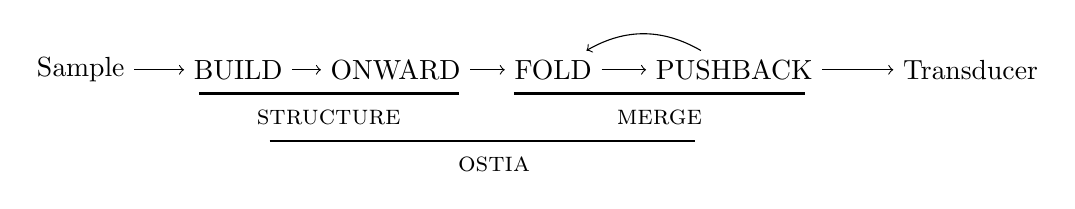
\begin{tikzpicture}
\node[]  at (0, 0) (s) {Sample};
\node[]  at (2, 0) (b) {BUILD};
\node[]  at (4, 0) (o) {ONWARD};
\node[]  at (6, 0) (f) {FOLD};
\node[]  at (8.3, 0) (p) {PUSHBACK};
\node[]  at (11.3, 0) (t) {Transducer};
\path[->]   (s) edge (b)
			(b) edge (o)
			(o) edge (f)
			(f) edge (p)
			(p) edge (t)
			(p) edge[bend right] (f);
\draw[thick] (1.5, -0.3) -- (4.8, -0.3);
\draw[thick] (5.5, -0.3) -- (9.2, -0.3);
\node[]  at (3.15, -0.6) {\textsc{structure}};
\node[]  at (7.35, -0.6) {\textsc{merge}};
\draw[thick] (2.4, -0.9) -- (7.8, -0.9);
\node[]  at (5.25, -1.2) {\textsc{ostia}};
\end{tikzpicture}
\caption{The main steps of OSTIA: \textsc{build}, \textsc{onward}, \textsc{fold} and \textsc{pushback}.}
\label{ostiamainsteps}
\end{figure}



\paragraph{BUILD}

The first step is to represent the input data using a transducer-like data structure.
For this purpose, we can build a \emph{prefix-tree transducer} that reads input strings of the training sample symbol-by-symbol, with the common prefixes of those strings stored in the states.
The initial state $q_\epsilon$ of such a PTT refers to the only common prefix of all the input strings: $\epsilon$.
The names of the later states refer to the common prefix those strings are sharing: the states accessible from the state $q_\epsilon$ correspond to different first symbols of the input strings.
So, for example, a state $q_{aba}$ reads a prefix \emph{aba} by passing through the following states: $q_\epsilon$, $q_{a}$, $q_{ab}$, and $q_{aba}$.
State outputs are set to the translations of the input strings that end up in that state.
For example, given the input pair $(ab, 01)$, we save $01$ in the state output of the state $q_{ab}$.

If the state output is not known, it is marked as $\perp$, or \emph{unknown}.
The unknown state output has two properties: \emph{absorbency} and \emph{neutrality}.
It is absorbent since its concatenation with any other string returns the same ``unknown'' output $\perp$.
It is neutral because the longest common prefix of any set of strings $W$ and $\perp$ is the same as the one of $W$ by itself, i.e.\  $\perp$ is transparent for this operation.
In such a way, the training sample provided to OSTIA is represented as a PTT.


\paragraph{ONWARD}

The outputs of the PTT are then modified to be \emph{onward}: such a PTT outputs translations as early as possible.
During this step, common prefixes of state outputs are pushed closer to the initial state.
For example, assume that the intermediate state of the PTT is the one as pictured in \ref{onwardgfsts} on the left side, with the onward version of that PTT on the right side.
In the input PPT, the state output of the state $q_a$ is $1$, and the translations on all edges coming out of $q_a$ ($q_a\xrightarrow{\text{a:10}}q_{aa}$ and $q_a\xrightarrow{\text{b:11}}q_{ab}$) also contain $1$ as their prefix.
Therefore, this prefix can be removed from the state output and transitions, and be introduced in the transducer earlier, namely, on the transition incoming into the state $q_a$.
Onwarding starts from the \emph{leaves} of the PTT (the nodes that do not have any outcoming arcs), and percolates to the initial state $q_\epsilon$.




\begin{figure}[h!] 
\centering
\begin{tikzpicture}
\node[state, initial]  at (0,1) (e) {$\epsilon:\epsilon$};
\node[state]  at (2,1) (a) {a:1};
\node[state]  at (4,2) (aa) {aa:$\epsilon$};
\node[state]  at (4,0) (ab) {ab:$\epsilon$};
\path[->] (e) edge[above] node{a:$\epsilon$} (a)
		  (a) edge[above] node{a:10} (aa)
		  (a) edge[above] node{b:11} (ab);
\end{tikzpicture}
%
\hspace{3em}
%
\begin{tikzpicture}
\node[state, initial]  at (0,1) (e) {$\epsilon:\epsilon$};
\node[state]  at (2,1) (a) {a:$\epsilon$};
\node[state]  at (4,2) (aa) {aa:$\epsilon$};
\node[state]  at (4,0) (ab) {ab:$\epsilon$};
\path[->] (e) edge[above] node{a:1} (a)
		  (a) edge[above] node{a:0} (aa)
		  (a) edge[above] node{b:1} (ab);
\end{tikzpicture}
\caption{Non-onward and onward PTTs that are otherwise equivalent.}
\label{onwardgfsts}
\end{figure}



\paragraph{FOLD}

Then, we try to merge every pair of states of the PTT.
If (a) the state outputs of $q$ and $q'$ are the same or are $\perp$, (b) all the incoming branches of $q'$ can be redirected to $q$, and (c) all outgoing branches from $q'$ are consistent with the outgoing branches of $q$, states $q$ and $q'$ are merged.
Consistency implies either having matching outgoing branches, a possibility to add a missing branch, or, if required, being able to successfully delay a part of the output during the \emph{pushback} step.
Folding one state into another decreases the size of the transducer, and shows that the learner generalized the pattern.


\paragraph{PUSHBACK}

The pushback operation checks if a part of the output can be delayed and therefore removed from some transitions.
If pushing back a portion of the output is possible, states $q$ and $q'$ considered during the previous \emph{merge} step are combined, otherwise, their merge is rejected.
For example, consider the FST on the left side in figure \ref{pushbackostia}.
Reading \emph{a} from the state $q_\epsilon$ yields the translation \emph{uv}.
However, as the machine on the right shows, the translation's suffix \emph{v} can be delayed to the state output of $q_a$ and all the transitions outgoing from $q_a$.
It could let the state $q_e$ be merged with some other state in the FST.
After the pushback, OSTIA returns to the merging step and checks if there are other pairs of states that could be merged.
When no such pairs remain, OSTIA outputs the FST.
In some sense, \emph{pushback} is the operation opposite to \emph{onward} since it delays the outputs, but the resulting FST is always onward.

\begin{figure}[h!] 
\centering
\begin{tikzpicture}
\node[state, initial]  at (0,1) (e) {$\epsilon:\epsilon$};
\node[state]  at (2,1) (a) {a:$\epsilon$};
\node[state]  at (4,2) (aa) {aa:$\epsilon$};
\node[state]  at (4,0) (ab) {ab:$\epsilon$};
\path[->] (e) edge[above] node{a:uv} (a)
		  (a) edge[above] node{a:$\epsilon$} (aa)
		  (a) edge[above] node{b:$\epsilon$} (ab);
\end{tikzpicture}
%
\hspace{3em}
%
\begin{tikzpicture}
\node[state, initial]  at (0,1) (e) {$\epsilon:\epsilon$};
\node[state]  at (2,1) (a) {a:v};
\node[state]  at (4,2) (aa) {aa:$\epsilon$};
\node[state]  at (4,0) (ab) {ab:$\epsilon$};
\path[->] (e) edge[above] node{a:u} (a)
		  (a) edge[above] node{a:v} (aa)
		  (a) edge[above] node{b:v} (ab);
\end{tikzpicture}
\caption{OSTIA pushes back the suffix \emph{v}.}
\label{pushbackostia}
\end{figure}


In such a way, OSTIA constructs a subsequential FST that generalizes the mapping from the input strings into their output representations.
Note, that as well as the subregular learning algorithms discussed earlier in Chapter $3$, OSTIA requires a sample of only positive data.%
\footnote{The algorithmic complexity of OSTIA is $\mathcal{O}(n^3(m + \mid\Sigma\mid) + nm\mid\Sigma\mid)$, where $n$ is the sum of the input string lengths, $m$ is the length of the longest output string, and $\Sigma$ is the input alphabet \citep{DeLaHiguera2010}.}
The next subsection presents the inference steps of this algorithm given a concrete example.



\subsection{The successful example}
\label{exam1}

Here, I discuss a slightly modified example of the OSTIA inference steps originally presented in \cite{DeLaHiguera2010}.
The task is to learn the following mapping: word-final $a$ is rewritten as $1$, non-word-final $a$ corresponds to $0$, and $b$ is always translated as $1$.
Notice, that this pattern can be viewed as a generalization of a linguistically-motivated process of word-final devoicing since it involves a segment changing its value to the opposite at the end of the word.
The training sample that I use in this example is enlarged in comparison to the one presented by \cite{DeLaHiguera2010}: it provides \emph{all} the necessary pairs that guarantee the extraction of the pattern.

\textbf{Sample} = {[}(b, 1), (a, 1), (aa, 01), (ab, 01), (aba, 011), (aaa, 001){]}


\paragraph{Step I.}

At first, OSTIA constructs a PTT representing the input sample.
This PTT reads the left sides of the training sample one symbol at a time.
For every string $w$ of the input pair ($w$, $o$), there exists a state $q_w$ with the state output $o$.
All transitions of this PTT output an empty string.
If there is a state $q_{w'}$ that does not correspond to any input string of the training sample, its state output is $\perp$.
For example, there is no empty string in the given sample, so the state output of $q_\epsilon$ is $\perp$.

%\begin{figure}[h!] 
%\centering
\begin{center}
\begin{tikzpicture}
\small
\node[state, initial]  at (0,0) (e) {$\epsilon:\perp$};
\node[state]  at (2,1) (a) {a:1};
\node[state]  at (2,-1) (b) {b:1};
\node[state]  at (4,2) (aa) {aa:01};
\node[state]  at (6,2) (aaa) {aaa:001};
\node[state]  at (4,0) (ab) {ab:01};
\node[state]  at (6,0) (aba) {aba:011};
\path[->] (e) edge[above] node{a:$\epsilon$} (a)
		  (e) edge[above] node{b:$\epsilon$} (b)
		  (a) edge[above] node{a:$\epsilon$} (aa)
		  (a) edge[above] node{b:$\epsilon$} (ab)
		  (aa) edge[above] node{a:$\epsilon$} (aaa)
		  (ab) edge[above] node{a:$\epsilon$} (aba);
\end{tikzpicture}
\end{center}
%\caption{After step I: constructing the PTT}
%\label{ostiastep1}
%\end{figure}

\paragraph{Step II.}

Then, this PTT is onwarded.
For example, consider the state $q_{aaa}$ with the state output $001$.
We can replace it by $\epsilon$, and instead move $001$ to the incoming arc therefore obtaining a transition $q_{aa}\xrightarrow{\text{a:001}}q_{aaa}$.
The longest common prefix of the modified transition and the state output of $q_{aa}$ is the longest common prefix of $01$ and $001$, and that $0$ can be moved to the output of the arc $q_{a}\xrightarrow{\text{a:0}}q_{aa}$.
Other leaves of the FST are processed similarly.
After this step, the input sample is represented as an onward PTT.

\begin{center}
\begin{tikzpicture}
\small
\node[state, initial]  at (0,0) (e) {$\epsilon:\perp$};
\node[state]  at (2,1) (a) {a:1};
\node[state]  at (2,-1) (b) {b:$\epsilon$};
\node[state]  at (4,2) (aa) {aa:1};
\node[state]  at (6,2) (aaa) {aaa:$\epsilon$};
\node[state]  at (4,0) (ab) {ab:$\epsilon$};
\node[state]  at (6,0) (aba) {aba:$\epsilon$};
\path[->] (e) edge[above] node{a:$\epsilon$} (a)
		  (e) edge[above] node{b:1} (b)
		  (a) edge[above] node{a:0} (aa)
		  (a) edge[above] node{b:01} (ab)
		  (aa) edge[above] node{a:01} (aaa)
		  (ab) edge[above] node{a:1} (aba);
\end{tikzpicture}
\end{center}

\paragraph{Step III.}

Next, we start the process of generalizing the obtained PTT by trying to merge pairs of its states.
States are colored in two colors: red and blue.
\emph{Red states} cannot be eliminated from the FST: they are crucial and therefore cannot be folded into any other state.
At first, only the initial state $q_\epsilon$ is colored red.
All states that can be reached in one step from the red states are colored blue.
The status of \emph{blue states} is unclear: either they will be folded into some red states, or they will eventually be re-colored red.
After a state was colored red, its immediate children are automatically added to the list of blue states.
In our example, two states are colored blue -- $q_a$ and $q_b$ -- since they can be reached from $q_\epsilon$ in one step.


%\begin{figure}[h!] 
%\centering
\begin{center}
\begin{tikzpicture}
\small
\node[state, initial, red]  at (0,0) (e) {$\epsilon:\perp$};
\node[state, blue]  at (2,1) (a) {a:1};
\node[state, blue]  at (2,-1) (b) {b:$\epsilon$};
\node[state]  at (4,2) (aa) {aa:1};
\node[state]  at (6,2) (aaa) {aaa:$\epsilon$};
\node[state]  at (4,0) (ab) {ab:$\epsilon$};
\node[state]  at (6,0) (aba) {aba:$\epsilon$};
\path[->] (e) edge[above] node{a:$\epsilon$} (a)
		  (e) edge[above] node{b:1} (b)
		  (a) edge[above] node{a:0} (aa)
		  (a) edge[above] node{b:01} (ab)
		  (aa) edge[above] node{a:01} (aaa)
		  (ab) edge[above] node{a:1} (aba);
\end{tikzpicture}
\end{center}
%\caption{After steps II and III: onwarding the PTT and coloring the states}
%\label{ostiastep23}
%\end{figure}

\paragraph{Step IV.}

Then, the algorithm considers pairs where one state is red and another one is blue and tries to fold the blue state into the red one.
Let us then fold the state $q_b$ into $q_\epsilon$.
At first, we check if the state outputs of $q_b$ and $q_\epsilon$ are compatible.
They are $\perp$ and $\epsilon$, and therefore could be merged: they are \emph{not different} due to the transparency of $\perp$, so we assign $\epsilon$ to the state output of $q_\epsilon$.
The transition coming to the state $q_b$ is re-directed into the state $q_\epsilon$ thus yielding a loop on that state.
There is no other sub-tree rooted in $q_b$, so folding $q_b$ into $q_\epsilon$ can be finalized, and $q_b$ is removed from the FST.

\begin{center}
\begin{tikzpicture}
\small
\node[state, initial, red]  at (0,1) (e) {$\epsilon:\epsilon$};
\node[state, blue]  at (2,1) (a) {a:1};
\node[state]  at (4,2) (aa) {aa:1};
\node[state]  at (6,2) (aaa) {aaa:$\epsilon$};
\node[state]  at (4,0) (ab) {ab:$\epsilon$};
\node[state]  at (6,0) (aba) {aba:$\epsilon$};
\path[->] (e) edge[above] node{a:$\epsilon$} (a)
		  (e) edge[loop above] node{b:1} (e)
		  (a) edge[above] node{a:0} (aa)
		  (a) edge[above] node{b:01} (ab)
		  (aa) edge[above] node{a:01} (aaa)
		  (ab) edge[above] node{a:1} (aba);
\end{tikzpicture}
\end{center}

\paragraph{Step V.}

After the state $q_b$ is eliminated, $q_a$ is the only blue state left.
We therefore consider merging $q_a$ into $q_\epsilon$.
However, these two states have different state outputs, and therefore it is impossible.
As the result, $q_a$ is re-colored red, and $q_{aa}$ and $q_{ab}$ accessible in one step from $q_a$ are colored blue.


%\begin{figure}[h!] 
%\centering
\begin{center}
\begin{tikzpicture}
\small
\node[state, initial, red]  at (0,1) (e) {$\epsilon:\epsilon$};
\node[state, red]  at (2,1) (a) {a:1};
\node[state, blue]  at (4,2) (aa) {aa:1};
\node[state]  at (6,2) (aaa) {aaa:$\epsilon$};
\node[state, blue]  at (4,0) (ab) {ab:$\epsilon$};
\node[state]  at (6,0) (aba) {aba:$\epsilon$};
\path[->] (e) edge[above] node{a:$\epsilon$} (a)
		  (e) edge[loop above] node{b:1} (e)
		  (a) edge[above] node{a:0} (aa)
		  (a) edge[above] node{b:01} (ab)
		  (aa) edge[above] node{a:01} (aaa)
		  (ab) edge[above] node{a:1} (aba);
\end{tikzpicture}
\end{center}
%\caption{After steps IV and V: folded $q_b$ into $q_\epsilon$ and re-colored the states}
%\label{ostiastep45}
%\end{figure}

\paragraph{Step VI.}

We then try to merge $q_\epsilon$ and $q_{aa}$, but it is not possible since they have different state outputs.
States $q_{a}$ and $q_{aa}$ could be merged because they have the same state output: $1$.
The outgoing arcs reading $a$ from these two states are different: one outputs $0$, and another outputs $01$.
However, the difference is the suffix $1$ that can be pushed further to the state output of $q_{aaa}$, therefore making those two transitions identical.
The arrow incoming to $q_{aa}$ is then re-directed to $q_{a}$, and $q_{aa}$ is eliminated from the list of states.

%\begin{figure}[h!] 
%\centering
\begin{center}
\begin{tikzpicture}
\small
\node[state, initial, red]  at (0,1) (e) {$\epsilon:\epsilon$};
\node[state, red]  at (2,1) (a) {a:1};
%\node[state, blue]  at (4,2) (aa) {aa:1};
\node[state]  at (6,2) (aaa) {aaa:1};
\node[state, blue]  at (4,0) (ab) {ab:$\epsilon$};
\node[state]  at (6,0) (aba) {aba:$\epsilon$};
\path[->] (e) edge[above] node{a:$\epsilon$} (a)
		  (e) edge[loop above] node{b:1} (e)
		  (a) edge[loop above] node{a:0} (a)
		  (a) edge[above] node{b:01} (ab)
%		  (aa) edge[above] node{a:01} (aaa)
		  (ab) edge[above] node{a:1} (aba);
\end{tikzpicture}
\end{center}
%\caption{After step VI: folded $q_{aa}$ into $q_{a}$}
%\label{ostiastep6}
%\end{figure}


\paragraph{Step VII.}

The state $q_{ab}$ is then folded into $q_{\epsilon}$.
The incoming arrow is re-directed to $q_{\epsilon}$, and $1$ is pushed back to state state output of $q_{aba}$.
Since $q_{ab}$ was merged with another state, it is eliminated from the machine.
This leaves no other blue states in the machine, and it signifies that OSTIA completed the inference.

%\begin{figure}[h!] 
%\centering
\begin{center}
\begin{tikzpicture}
\small
\node[state, initial, red]  at (0,1) (e) {$\epsilon:\epsilon$};
\node[state, red]  at (3,1) (a) {a:1};
\node[state]  at (6,2) (aaa) {aaa:1};
\node[state]  at (6,0) (aba) {aba:1};
\path[->] (e) edge[above,, bend left] node{a:$\epsilon$} (a)
		  (e) edge[loop above] node{b:1} (e)
		  (a) edge[loop above] node{a:0} (a)
		  (a) edge[above, bend left] node{b:01} (e);
\end{tikzpicture}
\end{center}
%\caption{After step VII: folded $q_{ab}$ into $q_{\epsilon}$}
%\label{ostiastep7}
%\end{figure}

\paragraph{Step VIII.}

All blue states are now eliminated from the machine.
However, the states that were never colored are still present.
In SigmaPie, the last step included in the \emph{OSTIA} algorithm is the elimination of the unaccessible states from the machine.
After those steps are completed, we obtain the FST visualized below.% in \ref{ostialaststep}.

%\begin{figure}[h!] 
%\centering
\begin{center}
\begin{tikzpicture}
\small
\node[state, initial]  at (0,0) (e) {$\epsilon:\epsilon$};
\node[state] at (3,0) (a) {a:1};
\path[->] (e) edge[loop above] node{b:1} (e)
	(e) edge[above, bend left] node{a:$\epsilon$} (a)
	(a) edge[below, bend left] node{b:01} (e)
	(a) edge[loop above] node{a:0} (a);
\end{tikzpicture}
\end{center}
%\caption{OSTIA: the resulting FST}
%\label{ostialaststep}
%\end{figure}


\subsection{The unsuccessful example}
\label{exam2}

Now, consider a pattern of \emph{unbounded tone plateauing} (UTP).
In a pattern like that, a sequence of low tones is converted to high if surrounded by high tones.
For example, inputs \emph{HLH} and \emph{HLLLH} are mapped to the outputs \emph{HHH} and \emph{HHHHH}, correspondingly.
When a low tone $L$ follows a high tone, it might be written as either $L$ or $H$ depending on the presence of another $H$ anywhere further in the input.
In other words, it requires an \emph{unbounded lookahead}.

Patterns requiring lookahead, such as UTP, are called \emph{unbounded circumambient processes} since the triggers are located on both sides of the undergoer, and they can be arbitrary far from it.
Unbounded circumambient processes are not subsequential \citep{Jardine2016}, and therefore it is expected that OSTIA is unable to capture UTP.
I show that OSTIA fails to learn UTP with the following sample.

\textbf{Sample} = {[}(HHH, HHH), (HHL, HHL), (HL, HL), (HLH, HHH), (HLL, HLL), (HLLH, HHHH){]}

\paragraph{Step I.}
At first, consider a PTT corresponding to the given training sample $S$.

\begin{center}
\begin{tikzpicture}
\small
\node[state, initial]  at (0,0) (e) {$\epsilon:\perp$};
\node[state]  at (2,0) (H) {H:$\perp$};
\node[state]  at (4,2.3) (HH) {HH:$\perp$};
\node[state]  at (7,3.5) (HHH) {HHH:HHH};
\node[state]  at (7,1.1) (HHL) {HHL:HHL};
\node[state]  at (4,-2.3) (HL) {HL:HL};
\node[state]  at (7,-1.1) (HLH) {HLH:HHH};
\node[state]  at (7,-3.5) (HLL) {HLL:HLL};
\node[state]  at (10,-3.5) (HLLH) {HLLH:HLLH};
\path[->] (e) edge[above] node{H:$\epsilon$} (H)
		(H) edge[left] node{H:$\epsilon$} (HH)
		(H) edge[left] node{L:$\epsilon$} (HL)
		(HH) edge[above] node{H:$\epsilon$} (HHH)
		(HH) edge[above] node{L:$\epsilon$} (HHL)
		(HL) edge[above] node{H:$\epsilon$} (HLH)
		(HL) edge[above] node{L:$\epsilon$} (HLL)
		(HLL) edge[above] node{H:$\epsilon$} (HLLH);
\end{tikzpicture}
\end{center}

\paragraph{Step II.}
Then, as previously, let us push the state outputs from the leaf nodes closer to the initial state $q_\epsilon$.
The resulting PTT is onward.

\begin{center}
\begin{tikzpicture}
\small
\node[state, initial]  at (0,0.25) (e) {$\epsilon:\perp$};
\node[state]  at (2,0.25) (H) {H:$\perp$};
\node[state]  at (4,1.9) (HH) {HH:$\perp$};
\node[state]  at (7,2.7) (HHH) {HHH:$\epsilon$};
\node[state]  at (7,1.1) (HHL) {HHL:$\epsilon$};
\node[state]  at (4,-1.4) (HL) {HL:L};
\node[state]  at (7,-0.6) (HLH) {HLH:$\epsilon$};
\node[state]  at (7,-2.2) (HLL) {HLL:LL};
\node[state]  at (10,-2.2) (HLLH) {HLLH:$\epsilon$};
\path[->] (e) edge[above] node{H:H} (H)
		(H) edge[left] node{H:H} (HH)
		(H) edge[left] node{L:$\epsilon$} (HL)
		(HH) edge[above] node{H:H} (HHH)
		(HH) edge[above] node{L:L} (HHL)
		(HL) edge[above] node{H:HH} (HLH)
		(HL) edge[above] node{L:$\epsilon$} (HLL)
		(HLL) edge[above] node{H:HHH} (HLLH);
\end{tikzpicture}
\end{center}

\paragraph{Step III.}

Next, we prepare to start folding states and sub-trees of the PTT into each other by coloring the states in red and blue.
As previously, the initial state $q_\epsilon$ is colored red, and the state $q_H$ available from $q_\epsilon$ in one step is colored blue.

\begin{center}
\begin{tikzpicture}
\small
\node[state, initial, red]  at (0,0.25) (e) {$\epsilon:\perp$};
\node[state, blue]  at (2,0.25) (H) {H:$\perp$};
\node[state]  at (4,1.9) (HH) {HH:$\perp$};
\node[state]  at (7,2.7) (HHH) {HHH:$\epsilon$};
\node[state]  at (7,1.1) (HHL) {HHL:$\epsilon$};
\node[state]  at (4,-1.4) (HL) {HL:L};
\node[state]  at (7,-0.6) (HLH) {HLH:$\epsilon$};
\node[state]  at (7,-2.2) (HLL) {HLL:LL};
\node[state]  at (10,-2.2) (HLLH) {HLLH:$\epsilon$};
\path[->] (e) edge[above] node{H:H} (H)
		(H) edge[left] node{H:H} (HH)
		(H) edge[left] node{L:$\epsilon$} (HL)
		(HH) edge[above] node{H:H} (HHH)
		(HH) edge[above] node{L:L} (HHL)
		(HL) edge[above] node{H:HH} (HLH)
		(HL) edge[above] node{L:$\epsilon$} (HLL)
		(HLL) edge[above] node{H:HHH} (HLLH);
\end{tikzpicture}
\end{center}

\paragraph{Step IV.}

The algorithm attempts to merge the blue state into the red state.
However, it is not possible to fold the sub-tree of $q_H$ into $q_\epsilon$.
It would cause the arrow $q_{HH}\xrightarrow{\text{L:L}}q_{HHL}$ to be changed to $q_{\epsilon}\xrightarrow{\text{L:L}}q_{HHL}$.
It means that states $q_{HHL}$ and $q_{HL}$ need to be merged since both of them would be available from $q_\epsilon$ by reading $L$, but it is not possible because the state outputs of $q_{HHL}$ and $q_{HL}$ are different: \emph{$\epsilon$} and \emph{L}, correspondingly.
Therefore the merge is rejected, and $q_H$ is colored red.
Its daughter nodes $q_{HH}$ and $q_{HL}$ are now blue.

\begin{center}
\begin{tikzpicture}
\small
\node[state, initial, red]  at (0,0.25) (e) {$\epsilon:\perp$};
\node[state, red]  at (2,0.25) (H) {H:$\perp$};
\node[state, blue]  at (4,1.9) (HH) {HH:$\perp$};
\node[state]  at (7,2.7) (HHH) {HHH:$\epsilon$};
\node[state]  at (7,1.1) (HHL) {HHL:$\epsilon$};
\node[state, blue]  at (4,-1.4) (HL) {HL:L};
\node[state]  at (7,-0.6) (HLH) {HLH:$\epsilon$};
\node[state]  at (7,-2.2) (HLL) {HLL:LL};
\node[state]  at (10,-2.2) (HLLH) {HLLH:$\epsilon$};
\path[->] (e) edge[above] node{H:H} (H)
		(H) edge[left] node{H:H} (HH)
		(H) edge[left] node{L:$\epsilon$} (HL)
		(HH) edge[above] node{H:H} (HHH)
		(HH) edge[above] node{L:L} (HHL)
		(HL) edge[above] node{H:HH} (HLH)
		(HL) edge[above] node{L:$\epsilon$} (HLL)
		(HLL) edge[above] node{H:HHH} (HLLH);
\end{tikzpicture}
\end{center}

\paragraph{Step V.}

The state $q_{HH}$ can be merged with $q_\epsilon$.
Indeed, the outgoing arcs reading and writing $H$ are present in both of these states, and the outgoing arc from $q_{HH}$ to $q_{HHL}$ is now re-directed and originates from $q_{\epsilon}$.
All the incoming arcs into the state $q_{HH}$ are re-directed to target $q_\epsilon$.
It created two outgoing from the state $q_\epsilon$ arrows reading $H$: $q_{\epsilon}\xrightarrow{\text{H:H}}q_{H}$ and $q_{\epsilon}\xrightarrow{\text{H:H}}q_{HHH}$, so $q_{HHH}$ needed to be folded into $q_{H}$.
Their state outputs are compatible since they are $\perp$ and $\epsilon$, therefore, the output of the state $q_{H}$ was rewritten to $\epsilon$.


\begin{center}
\begin{tikzpicture}
\small
\node[state, initial, red]  at (0,0) (e) {$\epsilon:\perp$};
\node[state, red]  at (2,0) (H) {H:$\epsilon$};
\node[state]  at (1.3,1.9) (HHL) {HHL:$\epsilon$};
\node[state, blue]  at (4,0) (HL) {HL:L};
\node[state]  at (7,0.8) (HLH) {HLH:$\epsilon$};
\node[state]  at (7,-0.8) (HLL) {HLL:LL};
\node[state]  at (10,-0.8) (HLLH) {HLLH:$\epsilon$};
\path[->] (e) edge[above, bend left] node{H:H} (H)
		(H) edge[below, bend left] node{H:$\epsilon$} (e)
		(H) edge[above] node{L:$\epsilon$} (HL)
		(e) edge[left] node{L:L} (HHL)
		(HL) edge[above] node{H:HH} (HLH)
		(HL) edge[above] node{L:$\epsilon$} (HLL)
		(HLL) edge[above] node{H:HHH} (HLLH);
\end{tikzpicture}
\end{center}

\paragraph{Step VI.}

The state $q_{HL}$ can be merged with neither $q_\epsilon$ nor $q_{H}$ because the arrows reading $L$ bring the machine to states with different state outputs.
While the state output of $q_{HLL}$ is $LL$, $q_{HL}$ and $q_{HHL}$ output $L$ and $\epsilon$, correspondingly.
Therefore $q_{HL}$ is colored red, and its children $q_{HLH}$ and $q_{HLL}$ are now blue.
Additionally, $q_{HHL}$ is also blue because it originates from the red state $q_\epsilon$.


\begin{center}
\begin{tikzpicture}
\small
\node[state, initial, red]  at (0,0) (e) {$\epsilon:\perp$};
\node[state, red]  at (2,0) (H) {H:$\epsilon$};
\node[state, blue]  at (1.3,1.9) (HHL) {HHL:$\epsilon$};
\node[state, red]  at (4,0) (HL) {HL:L};
\node[state, blue]  at (7,0.8) (HLH) {HLH:$\epsilon$};
\node[state, blue]  at (7,-0.8) (HLL) {HLL:LL};
\node[state]  at (10,-0.8) (HLLH) {HLLH:$\epsilon$};
\path[->] (e) edge[above, bend left] node{H:H} (H)
		(H) edge[below, bend left] node{H:$\epsilon$} (e)
		(H) edge[above] node{L:$\epsilon$} (HL)
		(e) edge[left] node{L:L} (HHL)
		(HL) edge[above] node{H:HH} (HLH)
		(HL) edge[above] node{L:$\epsilon$} (HLL)
		(HLL) edge[above] node{H:HHH} (HLLH);
\end{tikzpicture}
\end{center}

\paragraph{Step VII.}

The state $q_{HLH}$ is merged with $q_\epsilon$, and the only arrow incoming in $q_{HLH}$ from $q_{HL}$ is now targeting $q_\epsilon$.
Since the state output of $q_{HLH}$ was $\epsilon$ and the one of $q_\epsilon$ was unknown, it is now re-defined as $\epsilon$.

\begin{center}
\begin{tikzpicture}
\small
\node[state, initial, red]  at (0,0) (e) {$\epsilon:\epsilon$};
\node[state, red]  at (2,0) (H) {H:$\epsilon$};
\node[state, blue]  at (1.3,1.9) (HHL) {HHL:$\epsilon$};
\node[state, red]  at (4,0) (HL) {HL:L};
\node[state, blue]  at (6,0) (HLL) {HLL:LL};
\node[state]  at (9,0) (HLLH) {HLLH:$\epsilon$};
\path[->] (e) edge[above, bend left] node{H:H} (H)
		(H) edge[below, bend left] node{H:$\epsilon$} (e)
		(H) edge[above] node{L:$\epsilon$} (HL)
		(e) edge[left] node{L:L} (HHL)
		(HL) edge[above, bend left=60] node{H:HH} (e)
		(HL) edge[above] node{L:$\epsilon$} (HLL)
		(HLL) edge[above] node{H:HHH} (HLLH);
\end{tikzpicture}
\end{center}

\paragraph{Step VIII.}

The state $q_{HLL}$ cannot be merged with any red state.
Its state output differs from those of all the red states.
The state $q_{HLL}$ is thus colored red, and its daughter state $q_{HLLH}$ is blue.

\begin{center}
\begin{tikzpicture}
\small
\node[state, initial, red]  at (0,0) (e) {$\epsilon:\epsilon$};
\node[state, red]  at (2,0) (H) {H:$\epsilon$};
\node[state, blue]  at (1.3,1.9) (HHL) {HHL:$\epsilon$};
\node[state, red]  at (4,0) (HL) {HL:L};
\node[state, red]  at (6,0) (HLL) {HLL:LL};
\node[state, blue]  at (9,0) (HLLH) {HLLH:$\epsilon$};
\path[->] (e) edge[above, bend left] node{H:H} (H)
		(H) edge[below, bend left] node{H:$\epsilon$} (e)
		(H) edge[above] node{L:$\epsilon$} (HL)
		(e) edge[left] node{L:L} (HHL)
		(HL) edge[above, bend left=60] node{H:HH} (e)
		(HL) edge[above] node{L:$\epsilon$} (HLL)
		(HLL) edge[above] node{H:HHH} (HLLH);
\end{tikzpicture}
\end{center}

\paragraph{Step IX.}

The state $q_{HLLH}$ is then merged with $q_\epsilon$, and the arrow incoming in it from the state $q_{HLL}$ is re-directed.
At this moment it is already clear that the algorithm failed to learn the UTP pattern.
The learner memorized that one or two $L$ need to be substituted by $H$ if they are followed by $H$, but did not generalize it to an unbounded number of $L$s.

\begin{center}
\begin{tikzpicture}
\small
\node[state, initial, red]  at (0,0) (e) {$\epsilon:\epsilon$};
\node[state, red]  at (2,0) (H) {H:$\epsilon$};
\node[state, blue]  at (1.3,1.9) (HHL) {HHL:$\epsilon$};
\node[state, red]  at (4,0) (HL) {HL:L};
\node[state, red]  at (6,0) (HLL) {HLL:LL};
\path[->] (e) edge[above, bend left] node{H:H} (H)
		(H) edge[below, bend left] node{H:$\epsilon$} (e)
		(H) edge[above] node{L:$\epsilon$} (HL)
		(e) edge[left] node{L:L} (HHL)
		(HL) edge[above, bend left=60] node{H:HH} (e)
		(HL) edge[above] node{L:$\epsilon$} (HLL)
		(HLL) edge[above, bend left=60] node{H:HHH} (e);
\end{tikzpicture}
\end{center}


\paragraph{Step X.}

Finally, the only remaining state $q_{HHL}$ is merged with $q_\epsilon$, therefore, creating a loop that reads and writes $L$ on that state.
There are no other remaining blue states, and therefore the learner outputs the FST.


\begin{center}
\begin{tikzpicture}
\small
\node[state, initial]  at (0,0) (e) {$\epsilon:\epsilon$};
\node[state]  at (2,0) (H) {H:$\epsilon$};
\node[state]  at (4,0) (HL) {HL:L};
\node[state]  at (6,0) (HLL) {HLL:LL};
\path[->] (e) edge[above, bend left] node{H:H} (H)
		(H) edge[below, bend left] node{H:$\epsilon$} (e)
		(H) edge[above] node{L:$\epsilon$} (HL)
		(e) edge[loop above, left] node{L:L} (e)
		(HL) edge[above, bend left=60] node{H:HH} (e)
		(HL) edge[above] node{L:$\epsilon$} (HLL)
		(HLL) edge[above, bend left=60] node{H:HHH} (e);
\end{tikzpicture}
\end{center}

As one can see, this transducer does not represent the UTP pattern.
For example, it would re-write an input string \emph{HLHLH} as \emph{HHHLH} by passing through the following states: $q_{\epsilon}\xrightarrow{\text{H:H}}q_{H}\xrightarrow{\text{L:$\epsilon$}}q_{HL}\xrightarrow{\text{H:HH}}q_{\epsilon}\xrightarrow{\text{L:L}}q_{\epsilon}\xrightarrow{\text{H:H}}q_{H}$.
Indeed, UTP cannot be expressed using a subsequential function: it requires an unbounded lookahead \citep{Jardine2016}.


\section{Learning experiments}
\label{learningexperiments}

Here, I discuss the learning experiments that I used to explore the capacities of the OSTIA algorithm.
Interestingly, OSTIA performed extremely well ($100$\%) on one or more harmonies without blockers.
However, the blocking effect showed itself as a challenge for the learner: the accuracy was falling drastically with the increasing length of the evaluated strings.

In this chapter, in contrast to the previous one, the learner extracts the ``rewrite rules'' instead of acquiring well-formedness conditions.
Namely, the learner is given a pair of strings imitating the underlying representation (UR) and the surface form (SF), and its goal is to learn how to map one into another.
This allows us to explore the capacities of OSTIA when challenged with natural language-like patterns discussed in the previous chapter: single and double harmonic systems with or without blockers, and others.
The code behind the experiments is available on GitHub \href{https://github.com/alenaks/subregular-experiments}{\faGithub} \citep{GHsubex}.

Note, however, the critical importance of the concrete implementation for the results of OSTIA.
For example, the condition activating pushback is slightly different in various OSTIA's pseudocodes.
\cite{OncinaEtAl1993} in the original formulation of OSTIA execute the pushback step depending on the output of $q_a$ transitions being a prefix of the corresponding $q_b$ transitions.
The core architecture of their learner, however, is a bit different from the one described in this section since their learner necessarily annotates the data with the end-markers and uses this information for the inference steps.
\cite{DeLaHiguera2010} executes the pushback and folds the states $q_a$ and $q_b$ if all outgoing transitions from those states carry the same output.
As one can see, in this case, the pushback step would not be useful: if the outputs of the transitions are identical, there is no disagreeing affix to be pushed further in the FST.
In the errata for his book, \cite{DeLaHiguera2011} changes that condition to depend on the color of the states accessible from $q_b$.
The OSTIA version implemented and used in this chapter has its core architecture following \cite{DeLaHiguera2010}, but the condition is in line with \cite{OncinaEtAl1993}.
There is a multitude of different versions of pseudocodes, and, therefore, even more versions of the possible implementations.
Thus the results obtained in this chapter are specific to the concrete interpretation of the fold and pushback conditions and need to be tested with different perspectives as well.


\subsection{Experimental setup}

As before, the experiments include $3$ main steps: \emph{data generation}, \emph{learning}, and \emph{model evaluation}.
%In this case, however, there are no experiments targeting raw natural language data since to the best of my knowledge, there are no such datasets available where underlying representations are mapped to their surface forms.

At first, the training pairs were generated.
For example, assume that we are trying to learn a single vowel harmony without blockers, where vowels are $A = \{a, o\}$, and the only consonant is $x$ that is making this harmony long-distant.
The training sample will then contain pairs such as \emph{(xoxxAxAxxxA, xoxxoxoxxxo)} and \emph{(axAxAxxA, axaxaxxa)}, where $A$ refers to an underspecified harmonizing vowel.
The left side of every pair contains the ``underlying representation'', where only the value of the first vowel is established, and all the consecutive vowels are hidden and represented as the name of their harmonic set, in this case, $A$.
The right side contains the ``surface forms'', where all the vowels harmonize with each other.
Such training pairs were then fed to OSTIA that outputted an FST representing the pattern. 

To evaluate the performance of the obtained FST, following \cite{GildeaJurafsky1996}, I generated another set of pairs that are used as a testing sample.
I provided the left-hand sides of those pairs to the FST as input and observed if the output strings were the same as the right-hand sides of the testing sample.

I used two types of testing samples: one includes strings of the same length as the ones that were used for training, and the second one contains strings that are twice longer than the latter.
The test sets containing a longer strings helped me to explore how well OSTIA generalized the target pattern beyond memorization of the concrete shapes found in the training sample.


\subsection{Target patterns}

Among the patterns that I targeted while exploring the capacities of the learner, there were some local patterns such as word-final devoicing, different types of long-distance harmonies, and some circumambient and unattested patterns.
Below I explain the parameters that I considered when choosing the learning experiments, see the summary in figure \ref{typesofexperiments}.

\paragraph{Long-distance}
The difference between local and long-distance processes is one of the very important distinctions for phonology.
In the first case, the process is locally bounded, whereas, in the second one, it involves a potentially unbounded amount of the intervening material.
As I show in chapter 3, this difference is crucial for strictly local models.
They can evaluate local dependencies, but cannot capture long-distant ones.
As an example of a purely local process, I use the phenomenon of word-final devoicing.

\paragraph{Includes blockers}
The blocking effect is widely discussed in the phonological literature.
Harmony systems with and without blockers cannot always be modeled in the same way.
For example, in chapter 3, I show that strictly piecewise models can express multiple well-formedness conditions, but they cannot capture even simple cases of blocking effects.
In the sample of explored datasets, $3$ out of the $7$ employed harmonies involve blockers.

\paragraph{Multiple processes}
A model cannot always handle multiple processes at the same time.
For example, a single tier-based strictly local grammar can express a vowel or a consonant harmony, but it cannot capture both of them at the same time.
There are a total of $4$ harmonies that involve several harmonic spreadings, and $2$ of them exhibit a blocking effect.


\paragraph{Different undergoers}
Some models can express several spreadings at once if all the harmonizing features are spread among the same sets of elements.
For example, the only case when a tier-based strictly local grammar can capture the agreement in two features is when both features are affecting vowels.
Therefore, $2$ of the explored datasets present this type of a harmonic system, with and without a blocking effect.

\paragraph{Unbounded lookahead}
In subsection \ref{exam2}, I showed that processes that require an unbounded lookahead are not subsequential, and therefore cannot be learned by OSTIA.
Therefore, I use $2$ automatically generated datasets that exhibit circumambient patterns, and show that they cannot be learned by a subsequential learner.

\paragraph{Typologically attested}
Finally, I explore both typologically attested and unattested patterns.
All types of harmonic processes are indeed attested in natural languages, as well as the unbounded tone plateauing.
As an example of a typologically unattested pattern, I use the first-last harmony enforcing the agreement among the initial and the final vowels.
Two datasets are exhibiting the first-last harmony: one of them includes an unbounded lookahead, and the other one does not.


\begin{table}[h]
\centering
\scalebox{0.78}{%
\begin{tabular}{|c|c|c|c|c|c|}
\hline
\textbf{\begin{tabular}[c]{@{}c@{}}long-\\ distant\end{tabular}} & \textbf{\begin{tabular}[c]{@{}c@{}}includes\\ blockers\end{tabular}} & \textbf{\begin{tabular}[c]{@{}c@{}}multiple\\ processes\end{tabular}} & \textbf{\begin{tabular}[c]{@{}c@{}}different\\ undergoers\end{tabular}} & \textbf{\begin{tabular}[c]{@{}c@{}}unbounded\\ lookahead\end{tabular}} & 
\textbf{\begin{tabular}[c]{@{}c@{}}typologically\\ attested\end{tabular}} \\ \hline
\multicolumn{6}{|c|}{\large \textit{word-final devoicing}}    \\ \hline
\cellcolor{gray!50}\faTimes                                                               & \cellcolor{gray!50}\faTimes &  \cellcolor{gray!50}                                                                    \faTimes & \cellcolor{gray!50}\faTimes                                                                        &       \cellcolor{gray!50}\faTimes  & {\Large\faCheck}                                                                 \\ \hline
\multicolumn{6}{|c|}{\large \textit{a single vowel harmony without blocking}}                                                                                                                                                                                        \\ \hline
{\Large\faCheck}  & \cellcolor{gray!50}\faTimes & \cellcolor{gray!50}\faTimes                                                                       &   \cellcolor{gray!50}\faTimes                                                                      &         \cellcolor{gray!50}\faTimes  & {\Large\faCheck}                                                               \\ \hline
\multicolumn{6}{|c|}{\large \textit{a single vowel harmony with blocking}}                                                                                                                                                                                           \\ \hline
{\Large\faCheck} & {\Large\faCheck} & \cellcolor{gray!50}\faTimes                                                                       &     \cellcolor{gray!50}\faTimes                                                                    &         \cellcolor{gray!50}\faTimes  & {\Large\faCheck}                                                               \\ \hline
\multicolumn{6}{|c|}{\large \textit{several vowel harmonies without blocking}}                                                                                                                                                                                       \\ \hline
{\Large\faCheck} &  \cellcolor{gray!50}\faTimes & {\Large\faCheck}                                                                       &        \cellcolor{gray!50}\faTimes                                                                 &          \cellcolor{gray!50}\faTimes  & {\Large\faCheck}                                                              \\ \hline
\multicolumn{6}{|c|}{\large \textit{several vowel harmonies with blocking}}                                                                                                                                                                                          \\ \hline
{\Large\faCheck} &  {\Large\faCheck}                 &                                                                      {\Large\faCheck} &       \cellcolor{gray!50}\faTimes                                                                  &           \cellcolor{gray!50}\faTimes  & {\Large\faCheck}                                                             \\ \hline
\multicolumn{6}{|c|}{\large \textit{vowel harmony and consonant harmony without blocking}}                                                                                                                                                                           \\ \hline
{\Large\faCheck} &  \cellcolor{gray!50}\faTimes &{\Large\faCheck}                                                                       &  {\Large\faCheck}                                                                       &\cellcolor{gray!50}\faTimes  & {\Large\faCheck}                                                                        \\ \hline
\multicolumn{6}{|c|}{\large \textit{vowel harmony and consonant harmony with blocking}}                                                                                                                                                                              \\ \hline
{\Large\faCheck} & {\Large\faCheck}   & {\Large\faCheck} & {\Large\faCheck}                & \cellcolor{gray!50}\faTimes  & {\Large\faCheck}                                                                       \\ \hline
\multicolumn{6}{|c|}{\large \textit{unbounded tone plateauing}}                                                                                                                                                                                                      \\ \hline
{\Large\faCheck} & \cellcolor{gray!50}\faTimes & \cellcolor{gray!50}\faTimes                                                                       &       \cellcolor{gray!50}\faTimes                                                                   &{\Large\faCheck}  & {\Large\faCheck}                                                                        \\ \hline
\multicolumn{6}{|c|}{\large \textit{simple first-last harmony}}                                                                                                                                                                                                      \\ \hline
{\Large\faCheck} & \cellcolor{gray!50}\faTimes & \cellcolor{gray!50}\faTimes                                                                       &         \cellcolor{gray!50}\faTimes                                                                &               \cellcolor{gray!50}\faTimes &               \cellcolor{gray!50}\faTimes  \\ \hline
\multicolumn{6}{|c|}{\large \textit{complex first-last harmony}}                                                                                                                                                                                                     \\ \hline
{\Large\faCheck} &  \cellcolor{gray!50}\faTimes & \cellcolor{gray!50}\faTimes                                                                       &           \cellcolor{gray!50}\faTimes                                                              &   {\Large\faCheck} &               \cellcolor{gray!50}\faTimes                                                                                                                             \\ \hline
\end{tabular}}
\caption{Parameters of the explored natural language patterns.}
\label{typesofexperiments}
\end{table}

\subsection{Experiment 1: word-final devoicing}

The rule of word-final devoicing prohibits underlyingly voiced obstruents from being voiced at the end of the word.
So, for example, in German, word-final /b/, /d/, and /g/ are realized as [p], [t], and [k] \citep{Wiebke1995}.
While the word for `children' is \emph{Kinder}, its singular form is \emph{Kin[t]}, i.e.\ the underlyingly voiced segment is voiceless at the end of the word.


\paragraph{Encoding}

As previously in Chapter 3, I used $3$ elements to encode this pattern: $b$ corresponding to voiced obstruents, $p$ to their voiceless counterparts, and $a$ standing for any other sound.
Like this, I generated pairs such as \emph{(apab, apap), (aba, aba)} and \emph{(app, app)}, where every $b$ of the first word of the pair is rewritten as $p$ in the second one.


\paragraph{Results}

I produced $1,500$ pairs exhibiting word-final devoicing and used them to build an FST using OSTIA.
The obtained FST performed excellently on both testing samples.
The first testing sample contained strings $1$ to $5$ characters long, similar to the training sample.
The second testing sample contained longer strings, namely $5$ to $10$ characters.
The perfect score of the FST on both tests signifies that it correctly acquired the pattern.



\begin{table}[h!]
\centering
\resizebox{\linewidth}{!}{%
\begin{tabular}{|r|l|}
\hline
\textbf{Pattern:} & word-final devoicing  \\ \hline
\textbf{Training sample (info):} & $1500$ pairs, $1$ to $5$ characters long \\ \hline
\textbf{Testing sample 1 (info):} & $1000$ pairs, $1$ to $5$ characters long \\ \hline
\textbf{Testing 1, accuracy:}         & $100$\% \\ \hline
\textbf{Testing 1, predictions:}      & ('apaap', 'apaap'), ('bpaab', 'bpaap'), ('abppp', 'abppp'), ... \\ \hline
\textbf{Testing sample 2 (info):} & $1000$ pairs, $5$ to $10$ characters long \\ \hline
\textbf{Testing 2, accuracy:}         & $100$\% \\ \hline
\textbf{Testing 2, predictions:}      & ('pappbab', 'pappbap'), ('aapppbapbb', 'aapppbapbp'), ... \\ \hline
\textbf{Number of states:}      & $2$ \\ \hline
\textbf{Number of transitions:} & $5$ \\ \hline
\end{tabular}}
\caption{Results of OSTIA learning word-final devoicing.}
\end{table}

The FST outputted by OSTIA is fully interpretable.
It has $2$ states and $5$ transitions in-between them.
In such a machine, the first state corresponds to the state of not observing $b$, and the second state to keeping $b$ in memory.
If $a$ or $p$ follow the memorized $b$, that $b$ is outputted together with $a$ or $p$.
If another $b$ follows a $b$, only one $b$ is written.
If $b$ is a final character of the input sequence, $p$ is written instead by the state output of $q_{b}$.
The obtained machine exactly corresponds to the target generalization, see figure \ref{exp1fst}.


\begin{figure}[h!] 
\centering
\begin{tikzpicture}
\node[state, initial]  at (0,0) (e) {$\epsilon:\epsilon$};
\node[state] at (3,0) (b) {b:p};
\path[->] (e) edge[loop above] node{p:p} (e)
		  (e) edge[loop below] node{a:a} (e)
		  (e) edge[above, bend left] node{b:$\epsilon$} (b)
		  (b) edge[below, bend left] node{a:ba, p:bp} (e)
		  (b) edge[loop above] node{b:b} (b);
\end{tikzpicture}
\caption{FST for word-final devoicing obtained by OSTIA.}
\label{exp1fst}
\end{figure}


\subsection{Experiment 2: a single vowel harmony without blocking}

The next challenge for OSTIA is to learn a pattern of a single vowel harmony without blocking.
For example, in Finnish, vowels harmonize in fronting.
Let us generalize a harmonic system where a single feature is spread without the possibility of being blocked.


\paragraph{Encoding}

Such a pattern can be generalized to a system where among vowels $A = \{a, o\}$, either $o$ or $a$ can occur in a surface representation, but not both.
We can then refer to the underspecified vowel of the underlying representation as $A$.
In order to make the spreading long-distant, $x$ encodes the transparent element.
This encoding defines pairs such as \emph{(axAxxAAxx, axaxxaaxx)} and \emph{(xxoxxAxAxx, xxoxxoxoxx)}.


\paragraph{Results}

OSTIA induces the FST that correctly generalizes the pattern, therefore, scoring $100$\% on both testing samples.
The inferred FST has $4$ states and $14$ transitions in-between them.
It is depicted in figure \ref{exp2fst}: note, that this machine is not minimal, i.e.\ there are states that do not express any information significant for the rule of harmony.
For example, $q_{x}$ and $q_{xx}$ only keep track of one or two $x$.
After $a$ was observed and written in the translation, the machine moves to the state $q_{a}$ and any $A$ from the input side is written as $a$ on the output side.
Instead, observing $o$ keeps the FST in the initial state $q_{e}$, and any following $A$ is then re-written as $o$.
Such an FST, although not minimal, correctly captures the intended harmonic system.

\begin{table}[h!]
\centering
\resizebox{\linewidth}{!}{%
\begin{tabular}{|r|l|}
\hline
\textbf{Pattern:} & a single vowel harmony without blocking  \\ \hline
\textbf{Training sample (info):} & $5000$ pairs, $1$ to $10$ characters long \\ \hline
\textbf{Testing sample 1 (info):} & $1000$ pairs, $1$ to $10$ characters long \\ \hline
\textbf{Testing 1, accuracy:}         & $100$\% \\ \hline
\textbf{Testing 1, predictions:}      & ('oAxxxAxxx', 'ooxxxoxxx'), ('xxaAxxAAxA', 'xxaaxxaaxa'), ... \\ \hline
\textbf{Testing sample 2 (info):} & $1000$ pairs, $15$ to $20$ characters long \\ \hline
\textbf{Testing 2, accuracy:}         & $100$\% \\ \hline
\textbf{Testing 2, predictions:}      & ('oAxAAxxAAxxxAxAAxA', 'ooxooxxooxxxoxooxo'), ... \\ \hline
\textbf{Number of states:}      & $4$ \\ \hline
\textbf{Number of transitions:} & $14$ \\ \hline
\end{tabular}}
\caption{Results of OSTIA learning a single vowel harmony without blocking.}
\end{table}


\begin{figure}[h!] 
\centering
\begin{tikzpicture}
\node[state, initial]  at (0,0) (e) {$\epsilon:\epsilon$};
\node[state]  at (3,-2) (x) {x:$\epsilon$};
\node[state]  at (6,0) (xx) {xx:$\epsilon$};
\node[state]  at (3,-4) (a) {a:$\epsilon$};
\path[->] (e) edge[loop above] node{o:o} (e)
		(e) edge[above, bend left] node{A:o} (xx)
		(xx) edge[above] node{A:o, x:x, o:o} (e)
		(e) edge[left, bend right] node{a:a} (a)
		(xx) edge[right, bend left] node{a:a} (a)
		(e) edge[above, bend left] node{x:x} (x)
		(x) edge[above, bend left] node{A:o} (e)
		(x) edge[below] node{o:o, x:x} (xx)
		(x) edge[below] node{a:a} (a)
		(a) edge[loop below] node{A:a, x:x} (a);
\end{tikzpicture}
\caption{FST for a single vowel harmony without blocking obtained by OSTIA.}
\label{exp2fst}
\end{figure}



\subsection{Experiment 3: a single vowel harmony with blocking}

While the previous experiment explores the performance of OSTIA on a dataset exhibiting no blocking effect, this one adds it to the picture.
In this case, while vowels within a word need to agree with respect to a certain feature, a blocker stops the spreading and only allows for its particular value after itself.

\paragraph{Encoding}

This pattern can be encoded as earlier, by using a class of vowels $A = \{a, o\}$, but now only $a$ can be observed after the blocker $f$.
As before, $x$ stands for a transparent element.
This defines pairs such as \emph{(oxAA, oxoo)}, \emph{(xaxxAxxA, xaxxaxxa)} and \emph{(xoxxAxfxxAx, xoxxoxfxxax)}.

\paragraph{Results}
In this case, the performance of the learner was not perfect.
Namely, if faced with a testing sample where the length of the words is $1$ to $10$ characters, it performs with the accuracy of $99.2$\%.
While mostly predicting the correct forms, for example, it rewrites the underlying form \emph{oxAxAA} as \emph{oxoxooxf}, incorrectly adding two extra characters to the end of the word.
The accuracy falls when the length of the testing sample is increased to $15$-$20$ characters: it only predicts $91.2$\% of the correct transformations.

\begin{table}[h!]
\centering
\resizebox{\linewidth}{!}{%
\begin{tabular}{|r|l|}
\hline
\textbf{Pattern:} & a single vowel harmony with blocking  \\ \hline
\textbf{Training sample (info):} & $5000$ pairs, $1$ to $10$ characters long \\ \hline
\textbf{Testing sample 1 (info):} & $1000$ pairs, $1$ to $10$ characters long \\ \hline
\textbf{Testing 1, accuracy:}         & $99.2$\% \\ \hline
\textbf{Testing 1, predictions:}      &  ('oxAxAA', 'oxoxoo\textcolor{red!50!black}{xf}'), ('xfxxaxAAx', 'xfxxaxaax\textcolor{red!50!black}{x}'), ... \\ \hline
\textbf{Testing sample 2 (info):} & $1000$ pairs, $15$ to $20$ characters long \\ \hline
\textbf{Testing 2, accuracy:}         & $91.2$\% \\ \hline
\textbf{Testing 2, predictions:}      & ('xxxoxfAxxxffxAxxx', 'xxxoxf\textcolor{red!50!black}{xxaaxxxffxaxxx}'), ... \\ \hline
\textbf{Number of states:}      & $74$ \\ \hline
\textbf{Number of transitions:} & $247$ \\ \hline
\end{tabular}}
\caption{Results of OSTIA learning a single vowel harmony with blocking.}
\end{table}


The obtained machine is not correct since some of the surface forms that it predicts are wrong.
However, the machine encoding the target generalization can be represented as a simple FST with $3$ states, see figure \ref{exp2fstrr} for the expected result.
It raises a question of what obstructed the inference of that machine, and why it happened in any consecutive experiment targeting a harmonic system involving a blocking effect.
I leave this issue aside for now, and come back to it further in the very end of the section 4.2.13.

\begin{figure}[h!] 
\centering
\begin{tikzpicture}
\node[state, initial]  at (0,0) (e) {$\epsilon:\epsilon$};
\node[state]  at (3,1) (a) {a:$\epsilon$};
\node[state]  at (3,-1) (o) {o:$\epsilon$};
\path[->] (e) edge[loop above] node{x:x} (e)
		  (a) edge[loop above] node{A:a, f:f, x:x} (a)
		  (o) edge[loop below] node{A:o, x:x} (o)
		(e) edge[above] node{a:a} (a)
		(e) edge[below] node{o:o} (o)
		(o) edge[right] node{f:f} (a);
\end{tikzpicture}
\caption{The expected FST for a single vowel harmony with blocking.}
\label{exp2fstrr}
\end{figure}



\subsection{Experiment 4: several vowel harmonies without blocking}

While the previous two experiments modeled spreadings of a single feature, this experiment targets the agreement in several features.
For example, in Kyrgyz, vowels agree in backness and rounding.
Abstractly, these features can be referred to as [$\alpha$] and [$\beta$].
Thus all possible stems can be of $4$ different types [$-\alpha, -\beta$], [$-\alpha, +\beta$], [$+\alpha, -\beta$], and [$+\alpha, +\beta$].


\paragraph{Encoding}

Now, let us assume that the class of vowels includes $4$ elements $A = \{a, e, o, u\}$.
Every one of these options encodes a possible type of vowel in a well-formed surface form.
As previously, $x$ is a transparent element.
Such encoding defines pairs \emph{(xxoxxAAxAx, xxoxxooxox)} and \emph{(xxxaxAxxx, xxxaxaxxx)}, among others.





\paragraph{Results}

Although the inferred machine is large ($37$ states and $90$ transitions), it performs perfectly on both testing samples.
In both cases, none of the forms predicted by the FST were disharmonic.



\begin{table}[h!]
\centering
\resizebox{\linewidth}{!}{%
\begin{tabular}{|r|l|}
\hline
\textbf{Pattern:} & several vowel harmonies without blocking  \\ \hline
\textbf{Training sample (info):} & $5000$ pairs, $1$ to $10$ characters long \\ \hline
\textbf{Testing sample 1 (info):} & $1000$ pairs, $1$ to $10$ characters long \\ \hline
\textbf{Testing 1, accuracy:}         & $100$\% \\ \hline
\textbf{Testing 1, predictions:}      &  ('xxoxxAAxAx', 'xxoxxooxox'), ('xxxexAxxA', 'xxxexexxe'), ... \\ \hline
\textbf{Testing sample 2 (info):} & $1000$ pairs, $15$ to $20$ characters long \\ \hline
\textbf{Testing 2, accuracy:}         & $100$\% \\ \hline
\textbf{Testing 2, predictions:}      & ('xxoAxxxAAxxAxxxAAx', 'xxooxxxooxxoxxxoox'), ... \\ \hline
\textbf{Number of states:}      & $37$ \\ \hline
\textbf{Number of transitions:} & $90$ \\ \hline
\end{tabular}}
\caption{Results of OSTIA learning several vowel harmonies without blocking.}
\end{table}

Interestingly, the learned machine has $37$ states, whereas smaller versions can easily be constructed, see figure \ref{exp4rests}.
It requires additional investigation to understand the conditions that were not satisfied during OSTIA execution, therefore, yielding the machine with a greater number of states than possible.

\begin{figure}[h!] 
\centering
\begin{tikzpicture}
\node[state, initial]  at (0,0) (e) {$\epsilon:\epsilon$};
\node[state]  at (3,1.3) (o) {o:$\epsilon$};
\node[state]  at (3,0) (u) {u:$\epsilon$};
\node[state]  at (3,-1.3) (ee) {e:$\epsilon$};
\path[->] (e) edge[loop above] node{a:a, A:a, x:x} (e)
		  (o) edge[loop right] node{A:o, x:x} (o)
		  (u) edge[loop right] node{A:u, x:x} (u)
		  (ee) edge[loop right] node{A:e, x:x} (ee)
		  (e) edge[above] node{o:o} (o)
		  (e) edge[above] node{u:u} (u)
		  (e) edge[above] node{e:e} (ee);
\end{tikzpicture}
\caption{The expected FST for several vowel harmonies without blocking.}
\label{exp4rests}
\end{figure}


\subsection{Experiment 5: several vowel harmonies with blocking}

The next task included learning Turkish vowel harmony.
It enforces vowels to agree in backness and rounding.
While all vowels within a word agree in backness, only high vowels acquire the rounding value of a previous vowel.
For example, the word \emph{son-lar-\textturnm n} `end-\textsc{pl-gen}' exemplifies that a non-high vowel from the plural suffix cannot acquire a rounding feature from the previous vowel, and therefore cannot transmit it to the following high vowel.
However, in \emph{son-un} `end-\textsc{gen}', the high vowel is realized rounded because it is preceded by a rounded vowel.
In both words, all vowels agree in backness.
In such a system, non-high vowels have a double nature: they are undergoers for the backness harmony, however, behave as blockers for the rounding one.


\paragraph{Encoding}

In the abstract representation of this pattern, it is impossible to use fewer vowels than already employed by Turkish.
This harmony depends on $3$ features (backness, rounding, and height), and therefore the minimum amount of vowels to encode it is $2^3 = 8$.
Now, there are two classes of underspecified vowels in the URs of the strings: high ($H$) and low ($L$).
The training pairs look like \emph{(uxHxLxxLLxxHxxL, uxuxaxxaaxx\textturnm xxa)}: the initial underspecified vowel is high, and therefore it agrees in rounding with a previous back rounded vowel, becoming $u$.
The next underspecified vowel is low and therefore is realized as unrounded $a$.
After several other low vowels, another high one follows, but it is not rounded (\textturnm) since it follows a non-round vowel.
Similarly to the earlier experiments, $x$ is transparent and makes this harmony long-distant.
The rules below summarize how exactly the underspecified segments $H$ and $L$ are realized in the SFs.

\medskip

$L = 
\left\{
\begin{tabular}{@{}l@{}}
    \textrm{`a' if the previous vowel is `o', `u', `a' or `\textturnm'} \\
    \textrm{`e' if the previous vowel is `\"o', `\"u', `e' or `i'}
\end{tabular}
\right\}$

\medskip

$H = 
\left\{
\begin{tabular}{@{}l@{}}
    \textrm{`\textopeno' if the previous vowel is `a' or `\textturnm'} \\
    \textrm{`a' if the previous vowel is `e' or `i'} \\
    \textrm{`o' if the previous vowel is `o' or `u'} \\
    \textrm{`e' if the previous vowel is `\"o' or `\"u'}
\end{tabular}
\right\}$

\bigskip


\begin{table}[h!]
\centering
\resizebox{\linewidth}{!}{%
\begin{tabular}{|r|l|}
\hline
\textbf{Pattern:} & several vowel harmonies with blocking  \\ \hline
\textbf{Training sample (info):} & $5000$ pairs, $1$ to $10$ characters long \\ \hline
\textbf{Testing sample 1 (info):} & $1000$ pairs, $1$ to $10$ characters long \\ \hline
\textbf{Testing 1, accuracy:}         & $97.9$\% \\ \hline
\textbf{Testing 1, predictions:}      &  ('exLxHxL', 'exexixe'), ('x\"uxxLxHxxL', 'x\"uxxex\textcolor{red!75!black}{\"u}xxe'), ... \\ \hline
\textbf{Testing sample 2 (info):} & $1000$ pairs, $15$ to $20$ characters long \\ \hline
\textbf{Testing 2, accuracy:}         & $87$\% \\ \hline
\textbf{Testing 2, predictions:}      & ('uxHxLxxLLxxHxxL', 'uxuxaxxaaxx\textcolor{red!75!black}{uxxa}'), ... \\ \hline
\textbf{Number of states:}      & $107$ \\ \hline
\textbf{Number of transitions:} & $318$ \\ \hline
\end{tabular}}
\caption{Results of OSTIA learning several vowel harmonies with blocking.}
\end{table}

\paragraph{Results}

Given the data sample of $5,000$ words $1$ to $10$ characters long, OSTIA did not learn this harmonic pattern completely.
When evaluated using the test data of the same length as the one in the training sample, $97.9$\% of the predicted surface forms were as expected.
On a test sample with longer words, the accuracy decreased to $87$\%.
Such a model consistently makes incorrect predictions such as \emph{(uxHxLxxLLxxHxxL, uxuxaxxaaxx\textbf{u}xxa)}, where a rounded high vowel $u$ occurs after a non-rounded low vowel $a$, instead of the expected high vowel \textturnm.
Interestingly, the performance of the algorithm did not increase significantly with the increased size of the training sample. 



\subsection{Experiment 6: vowel and consonant harmonies without blocking}

Now, let us consider two simultaneous yet independent harmonies.
A frequent case is when there are two classes of harmonizing elements: consonants and vowels.
Such a pattern is attested in several Bantu languages (Kikongo, Kiyaka, Bukusu a.o.).


\paragraph{Encoding}
Let us assume that vowels agree in [$\alpha$], and consonants agree in [$\beta$].
Such system would need at least $2$ vowels and $2$ consonants: $A = \{a, o\}$ and $B = \{b, p\}$.
Note that a special transparent element is not necessary since the presence of vowels makes the consonant harmony long-distant, and vise versa.
This encoding defines pairs such as \emph{(aApBAA, aappaa)} and \emph{(boABBABA, boobbobo)}, where in URs, every non-initial value of consonants and vowels is hidden under the name of the corresponding harmonic set.


\paragraph{Results}

The learner easily inferred the simultaneous vowel and consonant harmonies and scored $100$\% on both tests.
The FST has $4$ states and $16$ transitions in-between them.
Notice, that so far, the performance of OSTIA is $100$\% in every case when harmony does not include the blocking effect since it also performed extremely well on a single or double vowel harmonic systems earlier.


\begin{table}[h!]
\centering
\resizebox{\linewidth}{!}{%
\begin{tabular}{|r|l|}
\hline
\textbf{Pattern:} & vowel and consonant harmonies without blocking \\ \hline
\textbf{Training sample (info):} & $5000$ pairs, $1$ to $10$ characters long \\ \hline
\textbf{Testing sample 1 (info):} & $1000$ pairs, $1$ to $10$ characters long \\ \hline
\textbf{Testing 1, accuracy:}         & $100$\% \\ \hline
\textbf{Testing 1, predictions:}      &  ('oApBAA', 'ooppoo'), ('boABBABA', 'boobbobo'), ... \\ \hline
\textbf{Testing sample 2 (info):} & $1000$ pairs, $15$ to $20$ characters long \\ \hline
\textbf{Testing 2, accuracy:}         & $100$\% \\ \hline
\textbf{Testing 2, predictions:}      & ('opBAABAABBAABBAA', 'oppoopooppooppoo'), ... \\ \hline
\textbf{Number of states:}      & $4$ \\ \hline
\textbf{Number of transitions:} & $16$ \\ \hline
\end{tabular}}
\caption{Results of OSTIA learning vowel and consonant harmonies without blocking.}
\end{table}

The inferred FST is visualized in figure \ref{exp6fst}.
It has $4$ states, and every state corresponds to a type of vowel and consonant in a stem.
In particular, $q_\epsilon$ corresponds to stems where the vowel and consonant values are $a$ and $p$; $q_o$ corresponds to $o$ and $p$; $q_b$ to $a$ and $b$; and, finally, $q_{ob}$ encodes stems with $o$ and $b$.


\begin{figure}[h!] 
\centering
\begin{tikzpicture}
\node[state, initial]  at (0,0) (e) {$\epsilon:\epsilon$};
\node[state]  at (6,0) (ob) {ob:$\epsilon$};
\node[state]  at (3,2) (o) {o:$\epsilon$};
\node[state]  at (3,-2) (b) {b:$\epsilon$};
\path[->] (e) edge[loop above] node{a:a, A:a} (e)
		(e) edge[loop below] node{p:p, B:p} (e)
		(o) edge[loop above] node{A:o, B:p, p:p} (o)
		(b) edge[loop below] node{A:a, B:b, a:a} (b)
		(ob) edge[loop above] node{A:o} (ob)
		(ob) edge[loop below] node{B:b} (ob)
		(e) edge[above, bend right] node{o:o} (o)
		(e) edge[below, bend left] node{b:b} (b)
		(o) edge[above, bend right] node{b:b} (ob)
		(b) edge[below, bend left] node{o:o} (ob);
\end{tikzpicture}
\caption{FST for vowel and consonant harmonies without blocking obtained by OSTIA.}
\label{exp6fst}
\end{figure}


\subsection{Experiment 7: vowel and consonant harmonies with blocking}

Let us add a blocking effect to the pattern from the previous experiment.
Earlier we saw that OSTIA performs extremely well on data exhibiting a harmonic system that does not involve blockers.
However, adding a blocking effect in all cases resulted in the obtained FST not scoring $100$\% on either of the training datasets.

\paragraph{Encoding}

Let us use the encoding as in the previous experiment, where a stem is able to ``pick'' one vowel from the set $A = \{a, o\}$ and one consonant from $B = \{b, p\}$.
Additionally, I will introduce a blocker $t$, after which $b$ cannot occur, and needs to be realized as $p$ instead.
Along with all pairs that are well-formed for the same pattern without the blocker, it also introduces pairs such as \emph{(abABAtAABAB, ababataapap)}, where $B$ is rewritten as $b$ before the blocker since it inherited its value from the initial consonant $b$, however, $B$ is realized as $p$ after the blocker $t$.


\paragraph{Results}

The performance of OSTIA on this dataset is far from perfect.
While it scores $96.4$\% on the testing sample that includes strings of the same length as the training ones, the accuracy falls to $77.4$\% when the length of the test words is doubled.
It goes along with the previous results showing that OSTIA fails to generalize a blocking effect.



\begin{table}[h!]
\centering
\resizebox{\linewidth}{!}{%
\begin{tabular}{|r|l|}
\hline
\textbf{Pattern:} & vowel and consonant harmonies with blocking \\ \hline
\textbf{Training sample (info):} & $5000$ pairs, $1$ to $10$ characters long \\ \hline
\textbf{Testing sample 1 (info):} & $1000$ pairs, $1$ to $10$ characters long \\ \hline
\textbf{Testing 1, accuracy:}         & $96.4$\% \\ \hline
\textbf{Testing 1, predictions:}      &  ('aApABB', 'aapapp'), ('pBtaA', 'pptaa'), ('tpaBBAtAt', 'tpappatat\textcolor{red!75!black}{tppa}'), ... \\ \hline
\textbf{Testing sample 2 (info):} & $1000$ pairs, $15$ to $20$ characters long \\ \hline
\textbf{Testing 2, accuracy:}         & $77.4$\% \\ \hline
\textbf{Testing 2, predictions:}      & ('pBaBABBABttttABABBAB', 'ppapappaptttt\textcolor{red!75!black}{opoppop}'), ... \\ \hline
\textbf{Number of states:}      & $101$ \\ \hline
\textbf{Number of transitions:} & $406$ \\ \hline
\end{tabular}}
\caption{Results of OSTIA learning vowel and consonant harmonies with blocking.}
\end{table}



\subsection{Experiment 8: unbounded tone plateauing}

Now, consider a circumambient pattern of \emph{unbounded tone plateauing} (UTP).
This pattern is observed in some Niger-Congo languages such as Luganda, where all low tones (L) are realized as high (H) if they are surrounded by high tones.
As section \ref{exam2} shows, that pattern is not learnable by OSTIA since circumambient dependencies require an unbounded lookahead, and therefore cannot be expressed as subsequential transducers \citep{Jardine2016}.

\paragraph{Encoding}
This process involves low tones ($L$) changing their value to high ($H$) if they are surrounded by high tones.
To encode this pattern, we can simply create pairs where the underlying stretches of $L$s are realized as $H$ in the surface forms if surrounded by high tones, such as \emph{(LHHLHH, LHHHHH)}.
In all other cases, the underlying and the surface representations match.

\begin{table}[h!]
\centering
\resizebox{\linewidth}{!}{%
\begin{tabular}{|r|l|}
\hline
\textbf{Pattern:} & unbounded tone plateauing \\ \hline
\textbf{Training sample (info):} & $5000$ pairs, $1$ to $10$ characters long \\ \hline
\textbf{Testing sample 1 (info):} & $1000$ pairs, $1$ to $10$ characters long \\ \hline
\textbf{Testing 1, accuracy:}         & $100$\% \\ \hline
\textbf{Testing 1, predictions:}      &  ('HHHHL', 'HHHHL'), ('LLLHL', 'LLLHL'), ('LHHLHH', 'LHHHHH'), ... \\ \hline
\textbf{Testing sample 2 (info):} & $1000$ pairs, $15$ to $20$ characters long \\ \hline
\textbf{Testing 2, accuracy:}         & $94.9$\% \\ \hline
\textbf{Testing 2, predictions:}      & ('HLLLLLLLLHHLHHH', 'H\textcolor{red!75!black}{LLLLLLLL}HHHHHH'), ... \\ \hline
\textbf{Number of states:}      & $32$ \\ \hline
\textbf{Number of transitions:} & $64$ \\ \hline
\end{tabular}}
\caption{Results of OSTIA learning UTP.}
\end{table}

\paragraph{Results}

The obtained FST performs extremely well on the test set where the length of the words is the same as in the training sample.
However, the accuracy falls to $94.9$\% when the length of the test words is doubled.
This suggests that instead of capturing the pattern, the resulting machine simply memorized long substrings of tones that can be observed in the input.
Indeed, UTP cannot be captured as a subsequential machine.

\subsection{Experiment 9: a ``simple'' first-last harmony}

Now, let us consider learning a typologically unattested pattern such as \emph{first-last harmony} \citep{Lai15}.
This pattern enforces agreement among the first and the last vowels, while nothing else needs to agree.
First, let us consider a case when vowels are always the first and last elements of the word.

\paragraph{Encoding}

The encoding involves vowels $a$ and $o$, and a transparent element $x$.
In this representation of the pattern, words always start and end with a vowel, therefore the sample pairs look as follows: \emph{(oaoxaa, oaoxao), (axooxa, axooxa)}, etc.
If a final vowel of the underlying representation disagrees with the initial vowel, it is rewritten to match the initial vowel.

\paragraph{Results}

Such a pattern is easily induced by OSTIA.
The obtained model scores $100$\% on both test datasets.
The FST is pretty small and therefore interpretable: it has only $5$ states and $14$ transitions.


\begin{table}[h!]
\centering
\resizebox{\linewidth}{!}{%
\begin{tabular}{|r|l|}
\hline
\textbf{Pattern:} & a ``simple'' first-last harmony \\ \hline
\textbf{Training sample (info):} & $5000$ pairs, $1$ to $6$ characters long \\ \hline
\textbf{Testing sample 1 (info):} & $1000$ pairs, $1$ to $6$ characters long \\ \hline
\textbf{Testing 1, accuracy:}         & $100$\% \\ \hline
\textbf{Testing 1, predictions:}      & ('oaoxaa', 'oaoxao'), ('axooxa', 'axooxa'), ('oo', 'oo'), ... \\ \hline
\textbf{Testing sample 2 (info):} & $1000$ pairs, $10$ to $15$ characters long \\ \hline
\textbf{Testing 2, accuracy:}         & $100$\% \\ \hline
\textbf{Testing 2, predictions:}      & ('aoaxoaaoaaaoxaa', 'aoaxoaaoaaaoxaa'), ... \\ \hline
\textbf{Number of states:}      & $5$ \\ \hline
\textbf{Number of transitions:} & $14$ \\ \hline
\end{tabular}}
\caption{Results of OSTIA learning a ``simple'' first-last harmony.}
\end{table}

This FST is visualized below.
After starting to process the input string in $q_\epsilon$, it moves to either $q_a$ or $q_o$ depending on the first vowel that it reads.
States $q_o$ and $q_{ao}$ handle strings that start and end with $o$; similarly, the agreement within words that start with $a$ is enforced by states $q_a$ and $q_{oa}$.
Note the similarity of these two branches with the way the word-final devoicing was encoded earlier in FST \ref{exp1fst}.
While the disagreeing vowel is deleted from the transitions incoming to the states $q_{oa}$ and $q_{ao}$, that vowel is returned if it is not final.
If that vowel was, in fact, the last element of the input word, the other, ``agreeing'' vowel is written instead by the corresponding state output.



\begin{figure}[h!] 
\centering
\begin{tikzpicture}
\node[state, initial]  at (0,0) (e) {$\epsilon:\epsilon$};
\node[state]  at (3,1) (o) {o:$\epsilon$};
\node[state]  at (3,-1) (a) {a:$\epsilon$};
\node[state]  at (6,1) (oa) {oa:o};
\node[state]  at (6,-1) (ao) {ao:a};
\path[->] (o) edge[loop above] node{o:o, x:x} (o)
		  (a) edge[loop below] node{a:a, x:x} (a)
		  (oa) edge[loop right] node{a:a} (oa)
		  (ao) edge[loop right] node{o:o} (ao)
		(e) edge[below] node{a:a} (a)
		(e) edge[above] node{o:o} (o)
		(o) edge[below, bend left] node{a:$\epsilon$} (oa)
		(oa) edge[below, bend left] node{o:ao, x:ax} (o)
		(a) edge[below, bend left] node{o:$\epsilon$} (ao)
		(ao) edge[below, bend left] node{a:oa, x:ox} (a);
\end{tikzpicture}
\caption{FST for a ``simple'' first-last harmony obtained by OSTIA.}
\label{exp9fst}
\end{figure}



\subsection{Experiment 10: a ``complex'' first-last harmony}

The previous experiment targeted a pattern of the first-last harmony, where all words started and ended with a vowel.
Indeed, OSTIA learned that pattern with the accuracy of $100$\%.
Now, let us challenge the learner with a more complicated version of this rule: in this case, words are also able to start and end with a transparent element, however, the first vowel of the word still agrees with the final vowel.


\paragraph{Encoding}

The training sample, apart from including everything possible for the previous experiment, also includes pairs where the forms have a sequence of initial or final $x$.
So, for example, pairs such as \emph{(xxoxoaooaxx, xxoxoaoooxx)} and \emph{(axxoxoxxx, axxoxaxxx)} are added to the training sample.
Now, not all input-output pairs begin and end with a vowel.


\paragraph{Results}

The performance of OSTIA is not perfect on either of the tests.
The score is $98.6$\% on the test set that includes strings of the same length as the training sample, while it falls to $28.1$\% on a test set that includes longer words.
While OSTIA learned the previous version of this pattern, it failed to generalize a more complicated one.
Indeed, this result is expected since this case of first-last harmony requires an unbounded lookahead: there can be an unbounded amount of intervening material between the final vowel and the end of the word.
Patterns like this are not subsequential.


\begin{table}[h!]
\centering
\resizebox{\linewidth}{!}{%
\begin{tabular}{|r|l|}
\hline
\textbf{Pattern:} & ``complex'' first-last harmony \\ \hline
\textbf{Training sample (info):} & $5000$ pairs, $1$ to $12$ characters long \\ \hline
\textbf{Testing sample 1 (info):} & $1000$ pairs, $10$ to $29$ characters long \\ \hline
\textbf{Testing 1, accuracy:}         & $98.6$\% \\ \hline
\textbf{Testing 1, predictions:}      & ('oxaxooxx', 'oxaxoo\textcolor{red!75!black}{oxxaxx}'), ('xxaoxxaaxx', 'xxaoxxa\textcolor{red!75!black}{xaxx}'). ... \\ \hline
\textbf{Testing sample 2 (info):} & $1000$ pairs, $15$ to $20$ characters long \\ \hline
\textbf{Testing 2, accuracy:}         & $28.1$\% \\ \hline
\textbf{Testing 2, predictions:}      &  ('ooxaxoxoo\textcolor{red!75!black}{axxxxxx}', 'ooxaxoxoox\textcolor{red!75!black}{x}'), ... \\ \hline
\textbf{Number of states:}      & $79$ \\ \hline
\textbf{Number of transitions:} & $235$ \\ \hline
\end{tabular}}
\caption{Results of OSTIA learning a ``complex'' first-last harmony.}
\end{table}




\subsection{Summary of the results}

In this section, I explored automatic extraction of different types of harmonic or other assimilation processes, both attested and non-attested in natural languages.
These patterns were word-final devoicing, single and several vowel harmonies with and without blocking, independent vowel and consonant harmonies with and without blocking, unbounded tone plateauing, and different kinds of first-last harmony.


In the previous chapter I evaluated how learners acquire the well-formedness conditions imposed on the given training sample.
Here, I discuss learning the observed \emph{transformations} using the OSTIA algorithm.
The training sample then consists of pairs of examples, where the first element of the pair stands for the underlying representation, and the second element is the corresponding surface form.
Given such automatically generated sets of examples (see the code on GitHub \href{https://github.com/alenaks/subregular-experiments}{\faGithub} \citep{GHsubex}), I explored if OSTIA is capable of extracting the generalized rule from it.


As the first step, I generated the training data using the extension of the codebase explained in the previous chapter in 3.1.3.
Then, I provided those pairs as a training sample to OSTIA.
To test the performance of the learned FST, I generated another set of pairs and provided the left sides of those pairs as input to that FST.
The accuracy of the learned model is the percentage of times the FST outputted the same surface form as the right-hand side of the generated test pair.
I tested the obtained model on two types of test samples: in the first test sample, the strings are of the same length as in the training sample, and in the second one, they are approximately twice as long.
The first test sample evaluates the ``baseline'' performance of the learned models, while the second one uses longer strings to see how well the pattern was generalized.

%I will reiterate the importance of the concrete implementation of OSTIA for the obtained results, already discussed in section \ref{learningexperiments}.
%In this particular implementation, I followed the core architecture outlined by \cite{DeLaHiguera2010}, with the pushback condition in line with \cite{OncinaEtAl1993}.
%Therefore to have a full picture, it is important to conduct similar experiments%
% using other possible versions of OSTIA.


\begin{table}[h!]
\centering
\resizebox{\linewidth}{!}{%
\begin{tabular}{|l|c|c|}
\hline
\multicolumn{1}{|c|}{\textbf{Experiments}}                  & \textbf{$\mid\textrm{w}_{\textrm{train}}\mid$ = $\mid\textrm{w}_{\textrm{test}}\mid$} & \textbf{$\mid\textrm{w}_{\textrm{train}}\mid$ = $2 \times \mid\textrm{w}_{\textrm{test}}\mid$} \\ \hline
\textit{E1: word-final devoicing}                           & \cellcolor{green!75!black}100\%                    & \cellcolor{green!75!black}100\%                    \\ \hline
\textit{E2: a single vowel harmony without blocking}        & \cellcolor{green!75!black}100\%                    & \cellcolor{green!75!black}100\%                    \\ \hline
\textit{E3: a single vowel harmony with blocking}           &  \cellcolor{green!75!black!50!yellow}99.2\%                   & \cellcolor{green!75!black!20!yellow}91.2\%                   \\ \hline
\textit{E4: several vowel harmonies without blocking}       & \cellcolor{green!75!black}100\%                    & \cellcolor{green!75!black}100\%                    \\ \hline
\textit{E5: several vowel harmonies with blocking}          &  \cellcolor{green!75!black!50!yellow}97.9\%                   & \cellcolor{green!75!black!20!yellow}87\%                     \\ \hline
\textit{E6: vowel and consonant harmonies without blocking} & \cellcolor{green!75!black}100\%                    & \cellcolor{green!75!black}100\%                    \\ \hline
\textit{E7: vowel and consonant harmonies with blocking}    &  \cellcolor{green!75!black!50!yellow}96.4\%                   & \cellcolor{red!85!black!30!white} 77.4\%                   \\ \hline
\textit{E8: unbounded tone plateauing}                      &\cellcolor{green!75!black} 100\%                    &\cellcolor{green!75!black!20!yellow} 94.9\%                   \\ \hline
\textit{E9: ``simple'' first-last harmony}                             &  \cellcolor{green!75!black}100\%                   &  \cellcolor{green!75!black}100\%                   \\ \hline
\textit{E10: ``complex'' first-last harmony}                             &  \cellcolor{green!75!black!50!yellow}98.6\%                   &  \cellcolor{red!85!black}28.1\%                   \\ \hline
\end{tabular}}
\caption{Results of the learning experiments using OSTIA.}
\label{ostiaresults}
\end{table}


Table \ref{ostiaresults} provides a summary of the results discussed in this section.
The first column describes the results of testing on the same-length testsets, while the second one summarizes the performance of the models on the strings that are approximately twice longer.
Out of $10$ experiments, OSTIA generalized $5$ patterns extremely well, so its performance is $100$\% on both test sets.
These experiments were word-final devoicing, single and several vowel harmonies, independent vowel and consonant harmony, and a ``simple'' version of the first-last harmony.
Interestingly, none of the successful experiments included a pattern with a blocking effect. 
In fact, on the datasets with blocking, OSTIA performed significantly worse, scoring $91.2$\%, $87$\%, and $77.4$\% during the evaluations that used longer words.
Unbounded circumambient processes are not subsequential \citep{Jardine2016}, so OSTIA expectedly did not learn UTP.
Finally, the ``complex'' version of first-last harmony is also beyond the capacities of this learner because it requires an unbounded lookahead: only $28.1$\% of the predicted transformations are indeed correct.

The current implementation of OSTIA cannot capture the blocking effect, as the experiments 3, 5 and 7 show.
Theoretically, this can be caused by 3 different reasons: the inability of the algorithm to learn the blocking effect, the absence of the crucially important data points, and the inability of the current implementation of the algorithm to learn the blocking effect.
The algorithm behind OSTIA is proven to be correct by \cite{OncinaEtAl1993}.
The average error was not decreasing with the increased number of the training examples, and that shows that the problem is not rooted in the absence of some pairs of examples.
It only leaves one source of the issue, namely, the concrete implementation of the algorithm.
Indeed, as I discuss in the beginning of the section \ref{learningexperiments}, different pseudocodes of OSTIA have different conditions behind the activation of the pushback module.
In future work, re-implementing OSTIA with different versions of that condition is necessary to find the concrete implementation that can learn the full class of subsequential functions in practice%
\footnote{For example, one can attempt the pushback and fold of the states $q_a$ and $a_b$ if the outputs of the transitions with the same input symbol originating in those states have a non-empty common prefix.
Preliminary results show that OSTIA implementing this condition is capable of learning the blocking effect; however, it does not perform well on local processes.}.


\section{Beyond OSTIA}

So far, I presented OSTIA as the only way to learn mappings.
Alternatively, one might want to either specify OSTIA given some concrete assumptions or to use other transduction learners.
OSTIA learns \emph{total} functions, i.e.\ functions that are defined for all possible values of their input.
However, natural language input to output mappings are not total: not all inputs can be mapped to their output counterparts because some forms simply do not exist.
This results in the learner never having a chance to satisfy a certain condition, and therefore it might not converge on the target FST.
Learners can be redefined with respect to the natural language restrictions in ways that use negative data, require a deterministic finite-state acceptor (DFA) corresponding to the input or output, or define different types of locality.
In this section, I discuss available extensions of OSTIA (OSTIA-D/R, OSTIA-N), other learning algorithms (SOSFIA, ISLFLA, OSLFIA), and propose some ideas for further learners.
To the best of my knowledge, the performance of other transduction learners on different datasets was not explored as of now, and it would be an interesting project to be carried out in future.



\subsection{Specifying OSTIA}

Earlier in this chapter, I discussed the main version of the OSTIA algorithm: it builds a prefix tree using the input sides of the training sample, and then folds some states one into another, therefore generalizing the pattern.
However, the FST extraction can be greatly simplified by providing some extra information about the shape of the input or output strings, as it is done in OSTIA-D, OSTIA-R, and OSTIA-DR, or by giving a sample of negative strings, as in OSTIA-N.

A transducer encodes a mapping.
But in some cases, this mapping is not defined for \emph{any} input string, but rather for a subset of the possible strings.
If the constraints on the input are available a priori, one might use a form of OSTIA that encodes \textbf{D}omain knowledge, or OSTIA-D \citep{OncinaVaro1996}.
It takes as input not only the training sample but also the DFA describing the language of the input strings.
If that information is available for the output strings of the intended mapping, then the \textbf{R}ange is defined a priori.
OSTIA-R requires a DFA describing the output language \citep{CastellanosEtAl1998}.
Consequently, OSTIA-DR takes advantage of both domain and range DFAs \citep{OncinaVaro1996}.

As another type of prior knowledge, OSTIA-N uses the \textbf{N}egative data \citep{OncinaVaro1996}.
Such a learner is given a set of well-formed pairs, as well as a set of input strings that should \emph{not} be translated by the learned machine.
While merging the states, OSTIA-N checks that none of the prohibited inputs obtained a translation.


\subsection{Fixing outputs of some input symbols}

We might have information about some of the outputs.
Namely, the outputs of some input symbols can be fixed thus accelerating the convergence if the learner explores all possible options.
For example, assume observing a pair \emph{(sim, seen)} in the training sample.
Based on exclusively this pair, we can construct a total of $35$ prefix tree-shaped FSTs with different output values of input symbols $s$, $i$ and $m$, see some of the machines in \ref{seemsin1}.
Some of these FSTs output the translation \emph{seen} as soon as they read $s$, some of them distribute the string among different transitions, some of them only have this string as the state output of $q_{sim}$, and so on.


\begin{figure}[h!] 
\centering
\begin{tikzpicture}
\node[state, initial]  at (0,0) (e) {$\epsilon:\epsilon$};
\node[state]  at (1.7, 0) (s) {s:$\epsilon$};
\node[state]  at (3.4, 0) (si) {si:$\epsilon$};
\node[state]  at (5.1, 0) (sim) {sim:$\epsilon$};
\path[->] (e) edge[above, bend left] node{s:seen} (s)
		  (s) edge[above, bend left] node{i:$\epsilon$} (si)
		  (si) edge[above, bend left] node{m:$\epsilon$} (sim);
\end{tikzpicture}
\vspace{0.5em}
\begin{tikzpicture}
\node[state, initial]  at (8,0) (e1) {$\epsilon:\epsilon$};
\node[state]  at (8+1.7, 0) (s1) {s:$\epsilon$};
\node[state]  at (8+3.4, 0) (si1) {si:$\epsilon$};
\node[state]  at (8+5.1, 0) (sim1) {sim:$\epsilon$};
\path[->] (e1) edge[above, bend left] node{s:s} (s1)
		  (s1) edge[above, bend left] node{i:ee} (si1)
		  (si1) edge[above, bend left] node{m:n} (sim1);
\end{tikzpicture}
\vspace{0.5em}
\begin{tikzpicture}
\node[state, initial]  at (0,-1.5) (e2) {$\epsilon:\epsilon$};
\node[state]  at (1.7, -1.5) (s2) {s:$\epsilon$};
\node[state]  at (3.4, -1.5) (si2) {si:$\epsilon$};
\node[state]  at (5.1, -1.5) (sim2) {sim:n};
\path[->] (e2) edge[above, bend left] node{s:seen} (s2)
		  (s2) edge[above, bend left] node{i:se} (si2)
		  (si2) edge[above, bend left] node{m:e} (sim2);

\end{tikzpicture}
\vspace{0.5em}
\begin{tikzpicture}
\node[state, initial]  at (8,-1.5) (e3) {$\epsilon:\epsilon$};
\node[state]  at (8+1.7, -1.5) (s3) {s:$\epsilon$};
\node[state]  at (8+3.4, -1.5) (si3) {si:$\epsilon$};
\node[state]  at (8+5.1, -1.5) (sim3) {sim:$\epsilon$};
\path[->] (e3) edge[above, bend left] node{s:$\epsilon$} (s3)
		  (s3) edge[above, bend left] node{i:$\epsilon$} (si3)
		  (si3) edge[above, bend left] node{m:seen} (sim3);
\end{tikzpicture}
\caption{Some of the FSTs that can be built from the pair \emph{(sim, seen)} in the ``unbiased'' way; to be contrasted with the following figure.}
\label{seemsin1}
\end{figure}

However, if it is known in advance that some of the outputs can be fixed, the number of such $4$-state FSTs processing \emph{(sim, seen)} decreases significantly.
For example, if the output of the input symbol $s$ is fixed to $s$, only $10$ machines are possible.
In all of them, a transition $q_\epsilon\xrightarrow{\text{s:s}}q_{s}$ is fixed to only read and output $s$.
The number of possible machines then decreases to $10$, see figure \ref{seemsin2}.

\begin{figure}[h!] 
\centering
\begin{tikzpicture}
\node[state, initial]  at (0,0) (e) {$\epsilon:\epsilon$};
\node[state]  at (1.7, 0) (s) {s:$\epsilon$};
\node[state]  at (3.4, 0) (si) {si:$\epsilon$};
\node[state]  at (5.1, 0) (sim) {sim:$\epsilon$};
\path[->] (e) edge[above, bend left] node{s:s} (s)
		  (s) edge[above, bend left] node{i:ee} (si)
		  (si) edge[above, bend left] node{m:n} (sim);

\end{tikzpicture}
\vspace{0.5em}
\begin{tikzpicture}

\node[state, initial]  at (8,0) (e1) {$\epsilon:\epsilon$};
\node[state]  at (8+1.7, 0) (s1) {s:$\epsilon$};
\node[state]  at (8+3.4, 0) (si1) {si:$\epsilon$};
\node[state]  at (8+5.1, 0) (sim1) {sim:en};
\path[->] (e1) edge[above, bend left] node{s:s} (s1)
		  (s1) edge[above, bend left] node{i:$\epsilon$} (si1)
		  (si1) edge[above, bend left] node{m:e} (sim1);
\end{tikzpicture}
\caption{Some of the FSTs that can be built from the pair \emph{(sim, seen)} if the output of the input symbol $s$ is fixed to the output symbol $s$.}
\label{seemsin2}
\end{figure}

Instead, if we fix the output of the symbol $i$ to $ee$, there will be only $2$ possible machines that employ $4$ states.
The output of $s$ would be $s$ in both cases, but the way of obtaining $n$ in the translation will differ: in one case, its source is the transition $q_{si}\xrightarrow{\text{m:n}}q_{sim}$, and in another case, it is the state output of $q_{sim}$ that yields $n$.

See the implementation of OSTIA with the possibility of fixing outputs of some input symbols on GitHub \href{https://github.com/alenaks/OSTIA/blob/master/ostia_biased_outputs.ipynb}{\faGithub} \citep{GHtoktrans}.
However, this solution is not applicable if there are processes happening across the ``fixed'' symbol.
If a metathesis occurs across some segment the output of which is fixed, extraction of this pattern becomes tricky.
For example, in an Austronesian language Hawu, some vowels undergo metathesis across a consonant \citep{Blust2012}.
In this case, fixing the output of that consonant will make it more complicated for the learner to discover the pattern.




\subsection{Other transduction learners}

In this chapter, I only discussed the learning results obtained by conducting toy learning experiments using OSTIA.
However, there are several other subsequential learners available in the literature.
One of them presents a different from OSTIA approach to the induction of subsequential transducers from the set of training pairs, and the other two rely on the particular assumptions about the shape of the dependencies encoded in the mapping.

\textbf{Structured Onward Subsequential Function Inference Algorithm} (SOSFIA) proposed by \cite{JardineEtAl2014} assumes the existence of the $k$-local DFA that helps to navigate through the input sides of the training pairs.
The learner then induces a subsequential function that reads the input strings one-by-one and outputs their translations.
The obtained FST is onward, i.e.\ at any step, the biggest known part of the output string is produced.


ISLFLA and OSLFIA encode assumptions about the sources of dependencies.
\textbf{Input Strictly Local Function Learning Algorithm} (ISLFLA) assumes that the translations only depend on the input string, i.e.\ there is enough information in the input itself to construct the translation \citep{ChandleeEtAl2014}.
\textbf{Output Strictly Local Function Inference Algorithm} (OSLFIA), on the contrary, considers both the input string and the currently known output prefix as sources of the information for the prediction of the next output symbol \citep{ChandleeEtAl2015}.
See chapter 2 for the examples of input/output local functions.
Both learners require some integer $k$ to be known a priori, and their first step is a constriction of $k$-local DFA accepting input or output strings.

An enlarged set of experiments needs to be used when exploring SOSFIA, ISLFLA and OSLFIA.
The expected result is that SOSFIA will learn all subsequential mappings (word final devoicing, all types of harmonies, and the ``simple'' case of vowel harmony).
However, OSLFIA and ISLFLA cannot learn processes where a potentially unbounded number of segments can intervene in-between two agreeing elements, because such processes are neither ISL nor OSL \citep{ChandleeEtAl2015}.
It would imply that those two learners only capture the word-final devoicing, and fail on all other experiments, see figure \ref{predictedoresults}.
Extending the list of the experiment by different local dependencies, such as metathesis, epenthesis, and deletion, would allow one to explore the practical capabilities of those learning algorithms better.



\begin{table}[h!]
\centering
\resizebox{\linewidth}{!}{%
\begin{tabular}{|l|c|c|c|}
\hline
\multicolumn{1}{|c|}{\textbf{Experiments}}                  & \textbf{SOSFIA} & \textbf{OSLFIA} & \textbf{ISLFLA} \\ \hline

\textit{E1: word-final devoicing} 
& \faThumbsOUp*                    
& \faThumbsOUp*           
&    \faThumbsOUp*      \\ \hline

\textit{E2: a single vowel harmony without blocking}
& \faThumbsOUp*                  
& \cellcolor{gray!50}\faTimes*            
& \cellcolor{gray!50}\faTimes*    \\ \hline

\textit{E3: a single vowel harmony with blocking}           
&  \faThumbsOUp*               
& \cellcolor{gray!50}\faTimes*
& \cellcolor{gray!50}\faTimes* \\ \hline

\textit{E4: several vowel harmonies without blocking}       
& \faThumbsOUp*                 
& \cellcolor{gray!50}\faTimes*         
&  \cellcolor{gray!50}\faTimes*   \\ \hline

\textit{E5: several vowel harmonies with blocking}          
&  \faThumbsOUp*                   
& \cellcolor{gray!50}\faTimes*      
&  \cellcolor{gray!50}\faTimes*      \\ \hline

\textit{E6: vowel and consonant harmonies without blocking} 
& \faThumbsOUp*                
& \cellcolor{gray!50}\faTimes*       
&  \cellcolor{gray!50}\faTimes*  \\ \hline

\textit{E7: vowel and consonant harmonies with blocking}    
&  \faThumbsOUp*          
& \cellcolor{gray!50}\faTimes*
&  \cellcolor{gray!50}\faTimes*  \\ \hline

\textit{E8: unbounded tone plateauing}                      
& \cellcolor{gray!50}\faTimes*
& \cellcolor{gray!50}\faTimes*
& \cellcolor{gray!50}\faTimes* \\ \hline

\textit{E9: ``simple'' first-last harmony}                            
&  \faThumbsOUp*
& \cellcolor{gray!50}\faTimes*  
& \cellcolor{gray!50}\faTimes*   \\ \hline

\textit{E10: ``complex'' first-last harmony}                             &  \cellcolor{gray!50}\faTimes*                
&  \cellcolor{gray!50}\faTimes*           
&  \cellcolor{gray!50}\faTimes*  \\ \hline

\end{tabular}}
\caption{Predicted results (marked as *) of the learning experiments using SOSFIA, OSLFIA and ISLFLA learning algorithms.}
\label{predictedoresults}
\end{table}


\subsection{Learning groups of transducers}

Currently, the transduction learners proposed in the literature have a goal of constructing a working generalized transducer based on the finite data sample.
Different algorithms perform different strategies of pattern recognition.
However, all of them have an assumption that the input sample is sufficiently representative.
This is a very strong requirement: a fully representative data sample is not always available.
For this reason, it is possible to think of an algorithm that instead of extracting a single machine, builds a class of machines that behave equally with respect to the training sample but are non-equivalent otherwise.

For example, consider a learning algorithm for a group of equivalent yet not identical input local FSTs.
Such FSTs only rely on the information available in the input to predict the output.
A learner could start by taking an input $k$-local subsequential transducer template with unfilled outputs of the transitions.
Then the transducer reads the input strings and saves all substrings of the corresponding translation string in the outputs of the transitions taken to read the input string.
If the transition was taken before, the algorithm intersects the set of substrings of the current translation with the set of saved candidates, therefore, leaving only the candidates that are consistent throughout the whole training sample.
After the training data is processed, the algorithm builds a set of transducers based on the obtained guesses for every transition.

For example, when the pair \emph{(ab, aab)} is provided as the input to the learner, two out of many guesses about the target FST would be either (1) outputting $ab$ if we read $b$ after an $a$, or (2) $a$ is translated to $aa$, and $b$ stays intact, see figure \ref{fig:two_opt}.
However, as soon as the training pair \emph{(a, aa)} is encountered, the first machine from Figure \ref{fig:two_opt} is rejected, leaving the second machine as the applicable candidate.

\begin{figure}[h!] 
\centering
\begin{tikzpicture}
\node at (-4,0) {(1)};
\node[state, initial]  at (0,0) (q0) {$q_0$};
\node[state] at (2,0) (q1) {$q_a$};
\node[state] at (4,0) (q2) {$q_b$};
\path[->] 	(q0) edge[above] node{$a:a$} (q1)
			(q1) edge[above] node{$b:ab$} (q2);
\end{tikzpicture}
\begin{tikzpicture}
\node at (-4,0) {(2)};
\node[state, initial]  at (0,0) (q0) {$q_0$};
\node[state] at (2,0) (q1) {$q_a$};
\node[state] at (4,0) (q2) {$q_b$};
\path[->] 	(q0) edge[above] node{$a:aa$} (q1)
			(q1) edge[above] node{$b:b$} (q2);
\end{tikzpicture}
\caption{Possible guesses of the transition that can be built after observing the pair \emph{(ab, aab)}.}
\label{fig:two_opt}
\end{figure}

Similarly to OSTIA-D and SOSFIA, such a learner needs to know a priori the DFA corresponding to the input side of the language.
Therefore, assume that we have the input $k$-local DFA pre-initialized.
Every transition $q$ of that DFA corresponds to the set $\Omega_q$, and that set is empty upon the initialization.
Then, we read one pair from the training sample.
If $\Omega_q$ of that transition is empty, we fill every state activated while reading the input string with all the substrings of the right side of the training pair.
If $\Omega_q$ is not empty, we intersect all substrings of the newly encountered output string with the guesses that those transitions contain.
After the whole training sample is processed, we can build all possible transducers based on the remaining guesses in $\Omega$ of the transitions.
Finally, we can run the input sides of the training pairs through the transducers again to validate that it predicts only correct outputs.

At the moment, the algorithm is implemented \href{https://github.com/alenaks/subregular-experiments/blob/master/ISL_group_learner.ipynb}{\faGithub} \citep{GHbrutefst}, but it has not been extensively tested or optimized yet.
Further work on this algorithm includes elaborate presentation of the pseudocode, evaluating its time complexity, improving the implementation, and testing its performance on language data, as well as presenting the proof of its correctness.


\section{Learning processes: summary}

In this chapter, I discussed the automatic extraction of subsequential finite-state transducers from a sample of input-output pairs.
Namely, I summarized the main steps of the OSTIA algorithm, presented two walk-through examples, demonstrated the results of the learning experiments, and proposed ways to go beyond OSTIA's performance.

The learning experiments targeted extraction of natural language-like patterns.
The training samples exhibited in simplified ways such typologically attested processes as word-final devoicing, one or multiple harmonies with and without blocking effect, and unbounded tone plateauing.
Additionally, OSTIA was presented with a dataset exemplifying the unattested pattern of first-last harmony.
OSTIA successfully learned the generalization behind word-final devoicing, all harmonies without a blocking effect, and a ``simple'' version of first-last harmony.
If the target pattern exhibited a blocking effect, however, it significantly decreased the accuracy of OSTIA.
Finally and expectedly, the generalizations behind tone plateauing and the ``complex'' version of first-last harmony remained unlearned since they involve an unbounded lookahead, so these patterns are not subsequential.
I provided the obtained FSTs where applicable, but that was not enough to explain the learning outcomes of some of the experiments.


A lot of questions remain unanswered.
Firstly, it is unclear what makes it impossible for OSTIA to learn even a simple case of harmony with a blocking effect.
Second, it is also important to test OSTIA on non-length preserving processes and other phonological phenomena such as epenthesis, deletion, and metathesis.
Finally, there are learners such as ISLFLA and OSLFIA that induce input and output-local functions \citep{ChandleeEtAl2014,ChandleeEtAl2015}, and their performance on natural language patterns needs to be evaluated as well.


In this chapter, I discussed learning \emph{transformations} that capture processes which change underlying representations into the corresponding surface forms.
Previously, chapter 3 discussed learners that are capable of modeling \emph{well-formedness conditions} imposed on languages.
Following this line of research helps us to explore the ways to create computational models of language, therefore giving an opportunity for insights into how languages work.

